% Chapter 1

\chapter{Grundlagen}
\label{Chapter1}
In diesem Kapitel werden viele wichtige Grundlagen vorgestellt, die in der ganzen Arbeit an verschiedenen Stellen benötigt werden. Zuerst werden wir im Detail die deterministische Klein-Gordon-Gleichung mit zugehöriger Existenztheorie präsentieren. Um eine numerischen numerischen Lösungsansatz für die KGG zu erhalten, wird anschließend das Operatorsplitting erläutert und auf die KGG angewandt. Schlussendlich erklären wir die Modellierung der stochastischen Klein-Gordon-Gleichung und bieten eine kurze Wiederholung von benötigten Begriffen aus der Stochastik und Statistik.

\section{Die Klein-Gordon-Gleichung}
Die für diese Arbeit grundlegende Gleichung ist die lineare Klein-Gordon-Gleichung in der Form
\begin{align}
\label{kgg}
\partialdtt{u}(t,x)&=\alpha \Laplace u(t,x) - \beta(x)u(t,x), \: t>0, \, x\in \Torus^d\\
u(0,x)&=u_0(x), \: x\in \Torus^d\\
\partialdt{u}(0,x)&=v_0(x), \: x\in \Torus^d
\end{align}
Dabei ist $\Laplace$ der Laplace-Operator im Ort $x$, definiert als
\[\Laplace=\frac{\text{d}^2}{\text{d}x^2_1}+\dots+\frac{\text{d}^2}{\text{d}x^2_d}.\]\\
Bevor wir Abhängigkeiten von einer Zufallsvariablen hinzufügen, ist es hilfreich, die Gleichung für deterministische Parameter besser zu verstehen. Diese Mühe ist nicht vergebens, da einige numerische Verfahren zur Bestimmung der Lösung der zufallsabhängigen Gleichung stark auf einem robusten und schnellen Löser der deterministischen Gleichung basieren. Dazu seien als Stichworte Monte-Carlo-Verfahren und Kollokationsverfahren genannt, die wir im späteren Verlauf genauer betrachten werden.
\subsection{Physikalische Definitionen}
Die KGG ist eine relativistische Feldgleichung, welche die Kinematik von spin-freien Teilchen, wie dem Pion, beschreibt. Auch das 2012 entdeckte Higgs-Boson ist ein spin-freies Teilchen, es ist jedoch noch unklar, ob es wirklich das von dem Standardmodell der Teilchenphysik vorhergesagte Teilchen ist und sich vom Standardmodell beschreiben lässt \autocite{cern2016}.\\
Dabei ist
\begin{itemize}
\item $\Torus=\R/(2\pi\Z)$ der skalierte eindimensionale Torus. Wir werden ab sofort die vereinfachte Darstellung $\Torus^d=(-\pi,\pi)^d$ mit periodischen Randbedingungen verwenden. Diese Skalierung des Torus ermöglicht das direkte Verwenden der schnellen Fourier-Transformation. Eine beliebige andere Skalierung des Torus ist jedoch ohne Beschränkung der Allgemeinheit möglich.
\item $\absolute{u(t,x)}^2$ physikalisch als Ladungsdichte des Teilchens zum Zeitpunkt $t$ und Ort $x$ interpretierbar \autocite{kleingordon2016}. 
\item $\alpha>0$ das Quadrat der Wellengeschwindigkeit.
\item $\beta(x)>0, \forall x\in \Torus^d,$ in der physikalischen Interpretation das Quadrat aus dem Produkt von quadratischer Wellengeschwindigkeit, Masse und inversem \sloppy{planckschem} Wirkungsquantum. Die Abhängigkeit des Potentialteils der KGG vom Ort $x$ ist dabei eine Verallgemeinerung der klassischen Gleichung.
\item die Differentialgleichung im Gegensatz zur physikalischen Darstellung reellwertig. Insbesondere fordern wir, dass $u$, $u_0$ und $v_0$ reellwertig und die Anfangswerte $u_0$ und $v_0$ periodisch in $(-\pi,\pi)^d$ sind.
\end{itemize}

\subsection{Existenztheorie}
Um den analytischen Rahmen für die Existenz und Eindeutigkeit von Lösungen der KGG zu schaffen werden wir die Halbgruppentheorie verwenden. Die verwendete Theorie ist übernommen aus \autocite{HundSchnau} und \autocite{EngelNagel}, dort finden sich auch weitere Details und Beweise der verwendeten Theoreme.
\begin{mathdef}
Sei der Raum der beliebig häufig differenzierbaren periodischen Funktionen definiert als
\[C_\text{per}^\infty (\Torus^d)\coloneqq \lbrace v\colon \Torus^d\to\R \mid v \text{ beliebig häufig stetig differenzierbar und periodisch in }[-\pi,\pi]^d\rbrace\]
Definieren wir zu $v\in C^\infty((-\pi,\pi)^d)$ und $k\in\N_0$ die Sobolev-Norm $\norm{v}_{k,2}$ durch
\[\norm{v}_{k,2}^2\coloneqq \sum_{|m|\le k}\norm{\dxp{v}{m}}_{L^2((-\pi,\pi)^d)}^2,\quad \text{Multiindex }\, |m|=m_1+\dots + m_d\]
so erhalten wir bei Verwendung der schwachen Ableitung und mit Vervollständigung die Sobolev-Räume $H^k((-\pi,\pi)^d)$.\\
Wir definieren einen abgeschlossenen Unterraum --und somit einen Banachraum-- des Sobolev-Raums $H^k((-\pi,\pi)^d)$ durch
\[H_\text{per}^k(\Torus^d)\coloneqq \text{Abschluss von } C_\text{per}^\infty(\Torus^d)\left(\subset C^\infty((-\pi,\pi)^d)\right) \text{ bezüglich der Norm von } H^k((-\pi,\pi)^d)\]
\end{mathdef}
Zunächst definieren wir die benötigte Halbgruppe $S(\cdot)$ und ihren Generator $A$.
\begin{mathdef}
Zu einem Banachraum $R$ heißt die Abbildung $S(\cdot)\colon \R_+\to L(R)$, die einer Zeit $t$ einen beschränken linearen Operator zuordnet, eine Operatorhalbgruppe, wenn
\[S(0)=I,\quad S(t+s)=S(t)S(s)\quad \forall t,s\ge 0\]
$S(\cdot)$ heißt $C_0$-Halbgruppe bzw. stark stetig, wenn zusätzlich gilt
\[\forall r\in R\colon S_r(\cdot)\colon \R_+\to R,\: t\mapsto S(t)r \text{ ist stetig}\]
Den Generator $A$ von $S(\cdot)$ erhält man, indem der Definitionsbereich definiert wird als
\[D(A)\coloneqq \lbrace r\in R\mid \text{ der Grenzwert } \lim\limits_{t\to0+}\frac{1}{t}(S(t)r-r)\text { existiert in }R\rbrace\]
und man anschließend für $r\in D(A)$ definiert
\[Ar\coloneqq \lim\limits_{t\to0+}\frac{1}{t}(S(t)r-r)\]
\end{mathdef}
Im folgenden Theorem wird die Verwendung der Halbgruppentheorie zum Erhalten von eindeutigen Lösungen der KGG klar. Inspiriert ist diese Betrachtungsweise durch den endlich dimensionalen Fall, wo $S(t)r=e^{At}r$ explizit über die Matrixexponentialfunktion gegeben ist.
\begin{maththeorem}[{\autocite[Proposition 2.8]{HundSchnau}}]
Ist $A$ Generator der $C_0$-Halbgruppe $S(\cdot)$ und $r\in D(A)$, dann ist für alle $t\ge 0\colon \,S(t)r\in D(A)$ und
\[v\colon \R_+\to R,\quad t\mapsto S(t)r\]
die eindeutige Lösung des Cauchy-Problems
\begin{equation}
\begin{split}
v'(t)&=Av(t),\quad t\ge 0\\
v(0)&=r
\end{split}
\end{equation}
\end{maththeorem}
Formulieren wir unsere KGG als ein Cauchy-Problem obiger Gestalt, so ist also nur noch zu zeigen, dass der Generator eine $C_0$-Halbgruppe generiert.\\
Den Generator $C=A+B$ der KGG teilen wir auf und erhalten zuerst den Teilgenerator $A$
\[A=\begin{pmatrix}0 & \kappa I\\ \alpha\Laplace & 0\end{pmatrix},\quad \kappa \in (0,1],\alpha>0\]
Wir definieren den Hilbertraum $R=H^1_\text{per}(\Torus^d)\times H^0_\text{per}(\Torus^d)$ mit zugehörigem leicht abgewandelten Skalarprodukt 
\[\langle \begin{pmatrix}v_1\\v_2\end{pmatrix}, \begin{pmatrix}w_1\\w_2\end{pmatrix}\rangle =\int_{[-\pi,\pi]^d}\alpha \nabla v_1\nabla w_1+\kappa v_2w_2dx\] 
\todo[inline]{Problem: Die zugehörige Norm ist nicht äquivalent zur Standardnorm des HRs, da Poincare mit periodischen RB Poincare nicht gilt.}
Es ist $D(A)=H^2_\text{per}(\Torus^d)\times H^1_\text{per}(\Torus^d)\subset R$ dicht in $R$, da bereits $C_\text{per}^\infty\times C_\text{per}^\infty\subset D(A)$ bezüglicher schwächerer Norm dicht in $R$ ist.\\
Stones Theorem besagt, dass $A$ genau dann eine $C_0$-Halbgruppe von unitären Operatoren generiert, wenn $A$ schiefadjungiert bezüglich des Skalarprodukt des Hilbertraums ist. Wir rechnen nach:
\begin{align*}
\langle A\begin{pmatrix}v_1\\v_2\end{pmatrix}, \begin{pmatrix}w_1\\w_2\end{pmatrix}\rangle
&=\langle \begin{pmatrix}\kappa v_2\\\alpha \Laplace v_1\end{pmatrix}, \begin{pmatrix}w_1\\w_2\end{pmatrix}\rangle\\
&=\int_{[-\pi,\pi]^d}\kappa \alpha \nabla v_2\nabla w_1 + \kappa \alpha \Laplace v_1 w_2dx\\
&\stackrel{\text{Green}}{=}-\int_{[-\pi,\pi]^d}\alpha\kappa v_2\Laplace w_1+ \alpha\kappa \nabla v_1\nabla w_2dx,\quad \text{da $v_1,v_2,w_1,w_2$ periodisch}\\
&=-\langle \begin{pmatrix} v_1\\ v_2\end{pmatrix}, \begin{pmatrix}\kappa w_2\\\alpha \Laplace w_1\end{pmatrix}\rangle=-\langle \begin{pmatrix}v_1\\v_2\end{pmatrix}, A\begin{pmatrix}w_1\\w_2\end{pmatrix}\rangle
\end{align*}
Um den vollen Generator $C$ der KGG zu erhalten benötigen wir noch den zweiten Teiloperator $B$ definiert durch
\[B=\begin{pmatrix}0 & (1-\kappa)I\\-\beta(x) & 0\end{pmatrix}\]
Dazu verwenden wir das Theorem über beschränkte Störungen eines stark stetigen Generators.
\begin{maththeorem}[{\autocite[Theorem 1.3, Kapitel III]{EngelNagel}}]
Ist $A$ Generator einer stark stetigen Halbgruppe $S(\cdot)$ mit Definitionsbereich $D(A)$ auf einem Banachraum $R$ und $B\colon R\to R$ ein beschränkter linearer Operator, so ist
$C=A+B$ mit $D(C)\coloneqq D(A)$ ebenfalls Generator einer stark stetigen Halbgruppe.
\end{maththeorem}
Wir verwenden daher den Banachraum $R_B=H_\text{per}^0\times H_\text{per}^0\supset R=H_\text{per}^1\times H_\text{per}^0$ mit der Norm 
\[\norm{\begin{pmatrix}v_1\\v_2\end{pmatrix}}_B^2=\int_{[-\pi,\pi]^d}v_1^2+v_2^2dx\le 
\norm{\begin{pmatrix}v_1\\v_2\end{pmatrix}}^2_{H_\text{per}^1\times H_\text{per}^0}\]
\todo[inline]{Wieder ist die Norm nicht äquivalent zu der aus $R$, aber $B$ ist kein Operator von $R\to R$ mit unserer Wahl von $R$.}
Dann gilt
\begin{align*}
\norm{B\begin{pmatrix}v_1\\v_2\end{pmatrix}}^2_B&=\int_{[-\pi,\pi]^d}(1-\kappa)^2v_2^2+(\beta(x))^2v_1^2dx\\
&\le c\int_{[-\pi,\pi]^d}v_1^2+v_2^2dx=c\norm{\begin{pmatrix}v_1\\v_2\end{pmatrix}}_B^2
\end{align*}
Insgesamt ist somit der Generator 
\[C=\begin{pmatrix}0 & I\\ \alpha\Laplace - \beta(x) & 0\end{pmatrix}\]
der Klein-Gordon-Gleichung Generator einer $C_0$-Halbgruppe und das zugehörige Cauchy-Problem besitzt eine eindeutige Lösung in $D(A)$. Dies impliziert auch eine eindeutige Lösung der KGG in $H_\text{per}^2(\Torus^d)$.
\subsection{Exakte Lösungen}
Für spezielle Konfigurationen der Parameter und Anfangswerte können wir exakte Lösungen angeben. Diese sind hilfreich, um die Korrektheit von Implementierungen schnell und zuverlässig testen zu können. Außerdem werden so schnell die Grenzen und eventuelle Schwächen der Verfahren für gut gestellte Probleme deutlich.\\[0.5cm]
Mithilfe des Separationsansatzes $u(t,x)=g(x)f(t)$ erhalten wir aus (\ref{kgg}) die Darstellung
\begin{equation*}
(\alpha\Laplace g(x)-\beta(x)g(x))f(t) = g(x)f''(t).
\end{equation*}
Diese können wir trennen und bekommen die zwei Differentialgleichungen
\begin{align*}
\alpha\Laplace g(x)-\beta(x)g(x)&=\lambda g(x), \: \lambda\in\R\\
\mu f(t)&=f''(t), \: \mu\in \R.
\end{align*}
Für $\beta(x) \equiv \beta>0$ ergibt sich das Eigenwertproblem $-\Laplace g(x)=-\frac{\beta + \lambda}{\alpha}g(x)$ mit periodischen Randbedingungen und eine lineare gewöhnliche Differentialgleichung.\\
Schlussendlich gewinnen wir daraus Lösungen für die ursprüngliche KGG. Die Anfangswerte $u_0$ und $v_0$ der KGG werden dann entsprechend passend gewählt.\\[1cm]
Beispiele für exakte Lösungen ($d=1$) sind
\begin{align*}
u(t,x)&=\sin(\lambda x)(c_1 \sin(\mu t) + c_2 \cos(\mu t)), \quad \mu^2=\beta+\alpha \lambda^2,\quad \beta(x)\equiv \text{const}\\ 
u(t,x)&=(c_1 \sin(\lambda x) + c_2 \cos(\lambda x))\sin(\mu t), \quad \mu^2=\beta+\alpha \lambda^2,\quad \beta(x)\equiv \text{const}\\
u(t,x)&=\exp(-\cos(x))\sin(\mu t), \quad \beta(x)=\mu^2+\cos(x)+\sin^2(x), \, \mu \in \R
\end{align*}
wobei $\lambda\in \pi\Z$ um die Periodizität zu gewährleisten und $c_1, c_2 \in \R$ frei wählbare Skalierungsfaktoren sind.\\
Diese Lösungen lassen sich auch auf höhere Dimensionen erweitern, beispielsweise
\begin{eqnarray}
u(t,x)=\exp(-\cos(x_1+\dots+x_d))\sin(\mu t)\\
\beta(x)=\mu^2+d(\cos(x_1+\dots+x_d)+\sin^2(x_1+\dots+x_d)), \, \mu\in\R \nonumber
\end{eqnarray}
Um einen kleinen Einblick in die Gestalt einer einfachen expliziten Lösung der KGG zu erhalten, sind in Abbildung \ref{fig:exactsolonedim} und \ref{fig:exactsoltwodim} die Lösungen mit Parametern $\alpha=1$, $\beta(x)=4+d(\cos(\sum_{j=1}^dx_j)+\sin^2(\sum_{j=1}^dx_j))$ zum Zeitpunkt $t=0.5$ dargestellt.
% Visualize exact solutions by giving two example plots
\begin{figure}[!htb]
\minipage{0.5\textwidth}
  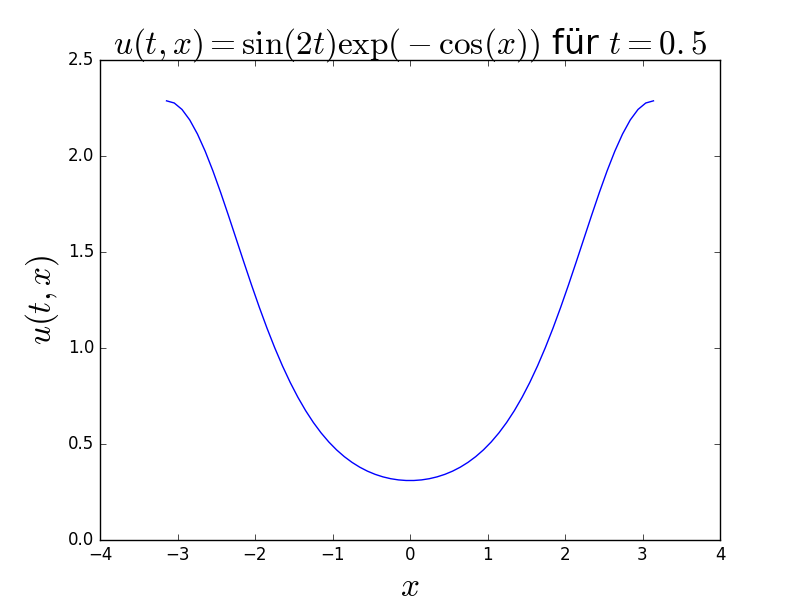
\includegraphics[width=\linewidth]{Figures/kgg_exact_solution_example1d.png}
  \caption{Exakte Lösung für $d=1$}
  \label{fig:exactsolonedim}
\endminipage
\minipage{0.5\textwidth}
  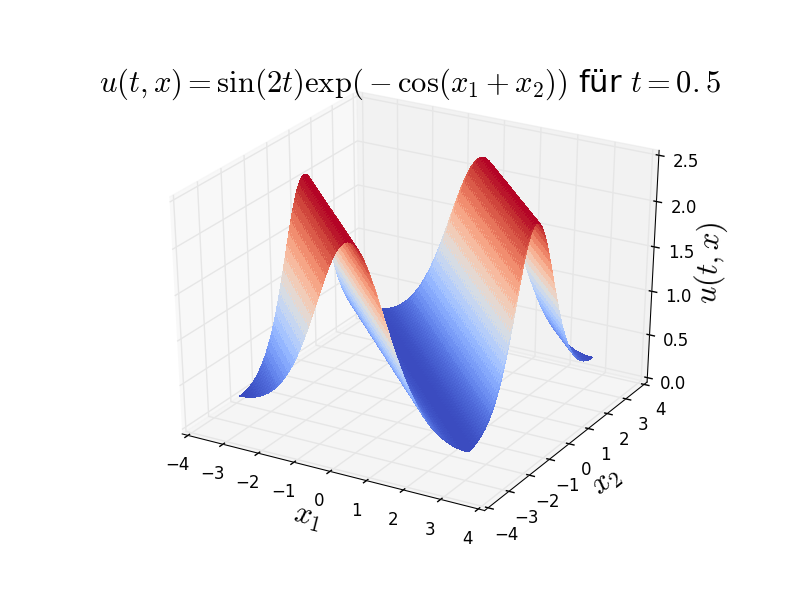
\includegraphics[width=\linewidth]{Figures/kgg_exact_solution_example2d.png}
  \caption{Exakte Lösung für $d=2$}
  \label{fig:exactsoltwodim}
\endminipage
\captionsetup{labelformat=empty}
\end{figure}

Eine Sammlung von nicht-periodischen Lösungen finden sich in \autocite{andreipolyanin2004}.

\section{Operatorsplitting}
Als numerischen Ansatz für approximative Lösungen der KGG wählen wir ein klassisches Operatorsplitting. Dabei wiederholen wir an dieser Stelle zuerst kurz die relevante Approximationstheorie und diskutieren mögliche Varianten.
\subsection{Grundlegende Idee}
Angenommen, wir stehen vor dem Problem die Differentialgleichung 
\begin{equation}
\label{gencompdgl}
\dt{u}(t)=(L+R)u(t), \, t>0, \quad u(0)=u_0
\end{equation}
lösen zu wollen. Dabei ist im einfachsten Fall $u$ eine vektorwertige Funktion und $L$ bzw. $R$ zwei Matrizen.\\
Ist beispielsweise $L=Q\Lambda Q^T$ eine einfach zu diagonalisierende Matrix und $R$ eine Diagonalmatrix, so sind die entkoppelten Gleichungen 
\begin{align*}
\dt{(Q^Tv)}(t)&=\Lambda Q^Tv(t), \quad v(0)=v_0\\
\dt{w}(t)&=Rw(t), \quad w(0)=w_0
\end{align*}
einfacher zu lösen als die Gleichung (\ref{gencompdgl}). Das Ziel des Operatorsplittings ist es, aus den Lösungen $v$ und $w$ eine Approximation an $u$ zu gewinnen.\\
Wir \emph{teilen} (engl. split) die Gleichung also in zwei neue Gleichungen auf. Häufig lässt sich dann eine der gewonnen Gleichungen sogar exakt lösen. Dieser Ansatz funktioniert auch für (nicht-lineare) Operatoren anstelle von Matrizen.\\
Diese zentrale Idee werden wir verwenden, um die KGG 
\begin{equation*}
\partialdtt{u}(t,x)=\alpha\Laplace u(t,x)-\beta(x)u(t,x)
\end{equation*}
zu splitten. Dabei wird der Operator $\alpha\Laplace$ in $L$ einfließen und $-\beta(x)$ in $R$. Man beachte jedoch, dass die zeitliche Ableitung zweiter Ordnung von $u$ eine Umschreibung in ein System erster Ordnung erfordert, bevor ein Splittingansatz sinnvoll ist.

\subsection{Lie-Trotter-Splitting}
\label{seclietrotter}
Wir beginnen mit einer rigorosen Einführung in Splittingverfahren. Als zentrales Ergebnis werden wir dabei das Strang-Splitting erhalten, welches einen Fehler $\mathcal{O}(\deltat^2)$ in Abhängigkeit von der Zeitschrittweite $\deltat$ besitzt.\\
Die folgende Einführung ist angelehnt an \autocite[Kapitel II.3 bis II.5]{HairerLubichWanner}.
\begin{mathdef}[Fluss einer Differentialgleichung]
Der Fluss $\varphi_t$ einer reversiblen Differentialgleichung
\begin{equation}
\label{orddgl}
\dt{y}=f(y),\quad y(0)\:\text{ gegeben}
\end{equation}
mit $f\colon \R^d\to\R^d$ ist die injektive Abbildung, die einem gegebenen $y_0$ die exakte Lösung $y(t)$ zum Zeitpunkt $t$ mit Anfangsbedingung $y(0)=y_0$ zuordnet. Also gilt
\begin{equation*}
\varphi_t(y_0)=y(t)\enspace und\enspace y(0)=y_0.
\end{equation*}
\end{mathdef}

Um Splittingverfahren von möglichst höher Ordnung zu bekommen ist es wichtig, die einzelnen Teilverfahren bestmöglich zu kombinieren. Hierbei spielt das adjungierte Verfahren eine wichtige Rolle, da es dabei hilft, symmetrisierte Verfahren mit gerader Ordnung zu gewinnen.
\begin{mathdef}[Adjungiertes Verfahren]
Ist $\Phi_{\deltat}\colon\R^d\to\R^d$ ein Einschrittverfahren so definieren wir das adjungierte Verfahren $\Phi_{\deltat}^*$ als das Inverse des Einschrittverfahrens mit negativer Schrittweite $\deltat$, also \[\Phi_{\deltat}^*\coloneqq\Phi_{-\deltat}^{-1}.\]
Das bedeutet, dass $y_1=\Phi_{\deltat}^*(y_0)$ implizit durch $\Phi_{-\deltat}(y_1)=y_0$ definiert wird.\\
Ist $\Phi_{\deltat}^*=\Phi_{\deltat}$ so nennen wir das Verfahren symmetrisch.
\end{mathdef}
Beispielsweise sind das explizite Euler-Verfahren $\Phi_{\deltat}^E$ und das implizite Euler-Verfahren $\Phi_{\deltat}^{IE}$ zueinander adjungiert: 
\[\Phi_{-\deltat}^E(y_1)=y_0\implies y_1+(-\deltat)f(y_1)=y_0\implies y_1=y_0+\deltat f(y_1)=\Phi_{\deltat}^{IE}(y_0)\] \\
Ohne Beweis sei bemerkt, dass $(\Phi_{\deltat}^*)^*=\Phi_{\deltat}$ und 
\begin{equation}
\label{adjlemma}
(\Phi_{\deltat}\circ \Psi_{\deltat})^*=\Psi_{\deltat}^* \circ \Phi_{\deltat}^*.
\end{equation}

\begin{mathdef}[Konsistenzordnung]
Eine numerische Methode zum Lösen von (\ref{orddgl}) ist (konsistent) von Ordnung $p$, wenn der lokale Fehler für hinreichend glattes $y$
\[\Phi_{\deltat}(y(t))=\varphi_{\deltat}(y(t))+\mathcal{O}(\deltat^{p+1})\] erfüllt.
\end{mathdef}
\begin{maththeorem}[Ordnung des adjungierten Verfahrens, vgl. 
{\autocite[Theorem II.3.2]{HairerLubichWanner}}]
\label{adjfloworder}
Sei $\varphi_t$ der exakte Fluss von (\ref{orddgl}) und sei $\Phi_{\deltat}$ ein Einschrittverfahren von Ordnung $p$ welches 
\[\Phi_{\deltat}(y_0)=\varphi_{\deltat}(y_0)+C(y_0)\deltat^{p+1}+\mathcal{O}(\deltat^{p+2})\]
erfüllt. Dann ist das adjungierte Verfahren $\Phi_{\deltat}^*$ ebenfalls von Ordnung $p$ und erfüllt
\[\Phi_{\deltat}^*(y_0)=\varphi_{\deltat}(y_0)+(-1)^{p}C(y_0)\deltat^{p+1}+\mathcal{O}(\deltat^{p+2})\]
Ist insbesondere $\Phi_{\deltat}$ symmetrisch, so ist wegen $C(y_0)=(-1)^pC(y_0)$ die Ordnung $p$ gerade.
\end{maththeorem}
Nun zerlegen wir die ursprüngliche Gleichung (\ref{orddgl}) in zwei Teile:
\[\dt{y}=f(y)=A(y)+B(y) \]
Das Aufteilen ist hierbei nicht eindeutig! Eine Möglichkeit im zweidimensionalen wäre zum Beispiel: $A=\text{P}_{(1,0)^T}f,\,B=\text{P}_{(0,1)^T}f$, wobei $\text{P}_v$ die Projektion auf $\text{span}(v)$ darstellt. Wie in unserem Fall der KGG ist die bereits vorhandene natürliche Aufteilung der Summe die Methode der Wahl.\\
Sind nun $\varphi_{\deltat}^A$ und $\varphi_{\deltat}^B$ die exakten Flüsse der Systeme
\begin{align}
\dt{y}&=A(y)\quad \text{und} \label{splitsimple1}\\ 
\dt{y}&=B(y) \label{splitsimple2}
\end{align}
so gewinnen wir daraus ein Verfahren zur Lösung der ursprünglichen Gleichung.\\
Hierzu starten wir von einem gegebenen Anfangswert $y_0$ und lösen das System (\ref{splitsimple1}) um einen Zwischenwert $y_{\onehalf}$ zu erhalten. Verwenden wir diesen als neuen Startwert für das System (\ref{splitsimple2}), so erhalten wir daraus einen Wert $y_1$, welcher eine Approximation an die Lösung $\varphi_{\deltat}(y_0)$ des ursprünglichen Systems ist.\\[1cm]
\noindent\begin{minipage}{0.3\textwidth}
\begin{tikzpicture}
  \matrix (m) [matrix of math nodes,row sep=3em,column sep=4em,minimum width=2em]
  {
     \, & y_1 \\
     y_0 & y_{\onehalf} \\};
  \path[-stealth]
    (m-2-1.east|-m-2-2) edge node [below] {$\varphi_{\deltat}^A$} (m-2-2)
    (m-2-2) edge node [right] {$\varphi_{\deltat}^B$} (m-1-2)
    (m-2-1) edge [dashed] node [above left] {$\Phi_{\deltat}$} (m-1-2);
\end{tikzpicture}
\begin{tikzpicture}
  \matrix (m) [matrix of math nodes,row sep=3em,column sep=4em,minimum width=2em]
  {
     y_{\onehalf} & y_1 \\
     y_0 & \, \\};
  \path[-stealth]
    (m-1-1.east|-m-1-2) edge node [above] {$\varphi_{\deltat}^A$} (m-1-2)
    (m-2-1) edge node [left] {$\varphi_{\deltat}^B$} (m-1-1)
    (m-2-1) edge [dashed] node [below right] {$\Phi_{\deltat}^*$} (m-1-2);
\end{tikzpicture}
\end{minipage}%
\hfill%
\begin{minipage}{0.7\textwidth}
Die Reihenfolge $A\to B$ ist willkürlich und kann auch umgekehrt werden. Tatsächlich sind die resultierenden Verfahren aufgrund von (\ref{adjlemma}) zueinander adjungiert, da der exakte Fluss wegen $y_1=\varphi_{-\deltat}^{-1}(y_0)=\varphi_{\deltat}^*(y_0)=\varphi_{\deltat}(y_0)$ als symmetrisches Einschrittverfahren auffassbar ist. Kurz:\\
\begin{align}
\label{liesplittings}
\Phi_{\deltat}=\varphi_{\deltat}^B \circ \varphi_{\deltat}^A\\
\Phi_{\deltat}^*=\varphi_{\deltat}^A \circ \varphi_{\deltat}^B\nonumber
\end{align} 
\end{minipage}

\begin{maththeorem}[Ordnung des Lie-Trotter-Splittings]
\label{lieorder1}
Das Lie-Trotter-Splitting $\Phi_{\deltat}=\varphi_{\deltat}^B \circ \varphi_{\deltat}^A$ und sein adjungiertes $\Phi_{\deltat}^*=\varphi_{\deltat}^A \circ \varphi_{\deltat}^B$ sind von Ordnung $p=1$.
\end{maththeorem}
\begin{proof}
Die Taylorreihe von $\varphi_{\deltat}$ lässt sich wegen 
\[\varphi_{\deltat}(y_0)=y(\deltat)=y(0)+\deltat \underbrace{y^\prime(0)}_{=f(y_0)}
+\frac{\deltat^2}{2}\underbrace{y^{\prime\prime}(0)}_{=f^\prime(y_0)y^\prime(0)=f^\prime(y_0)f(y_0)}+\mathcal{O}(\deltat^3)\] darstellen als 
\[\varphi_{\deltat}(y_0)=y_0+\deltat f(y_0)+\frac{\deltat^2}{2}f^\prime(y_0)f(y_0)+\mathcal{O}(\deltat^3)\]
Diese vergleichen wir nun mit der Taylorreihe des Splittings:
\begin{align*}
\left(\varphi_{\deltat}^B \circ \varphi_{\deltat}^A\right)(y_0)&=
\varphi_{\deltat}^B\left(y_0+\deltat f^A(y_0)+\frac{\deltat^2}{2}f^{\prime A}(y_0)f^A(y_0)+\mathcal{O}(\deltat^3)\right)\\
&=\left(y_0+\deltat f^A(y_0)+\frac{\deltat^2}{2}f^{\prime A}(y_0)f^A(y_0)\right)
+\deltat f^B\left(y_0+\deltat f^A(y_0)+\mathcal{O}(\deltat^2)\right)\\
&\quad+\frac{\deltat^2}{2}f^{\prime B}\left(y_0+\mathcal{O}(\deltat)\right)f^B\left(y_0+\mathcal{O}(\deltat)\right)+\mathcal{O}(\deltat^3)\\
&=y_0+\deltat f(y_0)+\frac{\deltat^2}{2}f^\prime(y_0)f(y_0)\\
&\quad+\frac{\deltat^2}{2}\left(f^{\prime B}(y_0)f^A(y_0)-f^{\prime A}(y_0)f^B(y_0)\right)+\mathcal{O}(\deltat^3)
\end{align*}
So erhalten wir für hinreichend glatte Funktionen $f^A$, $f^{\prime A}$, $f^B$ und $f^{\prime B}$ den Fehler \[\varphi_{\deltat}(y_0)-\left(\varphi_{\deltat}^B \circ \varphi_{\deltat}^A\right)(y_0)=\mathcal{O}(\deltat^2)\] und die Ordnung $p=1$. Mit Satz \ref{adjfloworder} ist das adjungierte Verfahren ebenfalls von Ordnung $p=1$.
\end{proof}

\subsection{Strang-Splitting}
\label{secstrang}
Durch geschicktes Kombinieren der Einschrittverfahren $\Phi_{\deltat}$ und $\Phi_{\deltat}^*$ mit verschiedenen Schrittweiten lassen sich Splittingverfahren beliebiger Ordnung konstruieren.
\begin{maththeorem}[vgl. {\autocite[Theorem II.4.1ff]{HairerLubichWanner}}]
Ist $\Phi_{\deltat}$ ein Einschrittverfahren von Ordnung $p$ so ist die Zerlegung
\[\Psi_{\deltat}=\Phi_{a_s\deltat}\circ \Phi_{b_s\deltat}^*\circ\dots\circ\Phi_{b_2\deltat}^*\circ\Phi_{a_1\deltat}\circ\Phi_{b_1\deltat}^*\]
von Ordnung $p+1$, wenn 
\begin{align*}
\sum_{j=1}^sa_j+b_j&=1\\
\sum_{j=1}^sa_j^{p+1}+(-1)^pb_j^{p+1}&=0
\end{align*}
\end{maththeorem}
Um das Lie-Trotter-Splitting zur Ordnung 2 zu erweitern motiviert der Satz die Wahl $\alpha_1=\beta_1=\onehalf$. Wir wollen nun ein Verfahren $\Phi_{\deltat}^S$ mit Ordnung $p=2$ gewinnen. Daher definieren wir
\[\Phi_{\deltat}^S=\Phi_{\deltathalf}^*\circ\Phi_{\deltathalf}=\left(\Phi_{\deltat}^S\right)^*\]
Wir erkennen sofort, dass es sich hierbei um ein symmetrisches Verfahren handelt. Als Komposition von Verfahren mit Ordnung 1 (siehe Satz \ref{lieorder1}) ist es ebenfalls mindestens von Ordnung 1. Als zusätzlich symmetrisches Verfahren gilt mit Satz \ref{adjfloworder}, dass das Verfahren mindestens von Ordnung 2 ist.\\
Dieses sogenannte \emph{Strang-Splitting} lässt sich unter Verwendung der aufgeteilten Flüsse (\ref{liesplittings}) auch darstellen als 

\noindent\begin{minipage}{0.3\textwidth}
\begin{tikzpicture}
  \matrix (m) [matrix of math nodes,row sep=3em,column sep=4em,minimum width=2em]
  {
  	 \, & y_{\frac{3}{4}} & y_1\\
     \, & y_{\frac{2}{4}} & \, \\
     y_0 & y_{\frac{1}{4}} & \,\\};
  \path[-stealth]
    (m-3-1.east|-m-3-2) edge node [below] {$\varphi_{\deltathalf}^A$} (m-3-2)
    (m-3-2) edge node [right] {$\varphi_{\deltathalf}^B$} (m-2-2)
    (m-3-1) edge [dashed] node [above left] {$\Phi_{\deltat}$} (m-2-2)
    
    (m-1-2.east|-m-1-3) edge node [above] {$\varphi_{\deltathalf}^A$} (m-1-3)
    (m-2-2) edge node [left] {$\varphi_{\deltathalf}^B$} (m-1-2)
    (m-2-2) edge [dashed] node [below right] {$\Phi_{\deltat}^*$} (m-1-3);
\end{tikzpicture}
\end{minipage}%
\hfill%
\begin{minipage}{0.7\textwidth}
\begin{align}
\Phi_{\deltat}^S&=\varphi_{\deltathalf}^A\circ\varphi_{\deltathalf}^B\circ\varphi_{\deltathalf}^B\circ\varphi_{\deltathalf}^A\nonumber\\
&=\varphi_{\deltathalf}^A\circ\varphi_{\deltat}^B\circ\varphi_{\deltathalf}^A
\end{align}
\end{minipage}
Für einen Schritt des Verfahrens ist wegen der Zusammenfassung der zwei inneren Teilschritte $\varphi_{\deltathalf}^B$ ist im Vergleich zum Lie-Trotter-Splitting also nur der anderthalbfache Aufwand nötig, aber man gewinnt bereits eine Ordnung dazu. Die Laufzeit kann sogar noch verbessert werden:\\
Gegeben sei ein Anfangswert $y_0$ für das System (\ref{orddgl}). Ist man an einer Approximation $y_T$ der Lösung $y(T)$ zu einem Zeitpunkt $T=n\deltat>0$ interessiert, so gilt unter Verwendung des Strang-Splittingverfahrens
\begin{align*}
y_T&=\underbrace{\Phi_{\deltat}^S\circ\dots\circ\Phi_{\deltat}^S}_{n\text{ mal}}(y_0)\\
&=\left(\varphi_{\deltathalf}^A\circ\varphi_{\deltat}^B\circ\varphi_{\deltathalf}^A\right)\circ\left(
\varphi_{\deltathalf}^A\circ\varphi_{\deltat}^B\circ\varphi_{\deltathalf}^A\right)\circ\dots\circ\left(
\varphi_{\deltathalf}^A\circ\varphi_{\deltat}^B\circ\varphi_{\deltathalf}^A\right)\\
&=\varphi_{\deltathalf}^A\circ\varphi_{\deltat}^B\circ\left(\varphi_{\deltat}^A\circ\varphi_{\deltat}^B\right)\circ\left(\varphi_{\deltat}^A\circ\varphi_{\deltat}^B\right)\circ\dots\circ\left(\varphi_{\deltat}^A\circ\varphi_{\deltat}^B\right)\circ\varphi_{\deltathalf}^A\\
&=\varphi_{\deltathalf}^A\circ\varphi_{\deltat}^B\circ
\underbrace{\Phi_{\deltat}^*\circ\dots\circ\Phi_{\deltat}^*}_{n-1\text{ mal}}\circ\,\varphi_{\deltathalf}^A
\end{align*}
Durch das Kombinieren der äußeren Halbschritte bekommt man somit eine Darstellung des Strang-Splittings, die im Vergleich zum Lie-Trotter-Splitting nur einen zusätzlichen Fluss berechnen muss und trotzdem Ordnung $p=2$ besitzt. Man muss hierbei allerdings auf Zwischenergebnisse verzichten, da diese eine weitere Anwendung von $\varphi_{\deltathalf}^A$ benötigen würden.\\[0.5cm]
Bisher sind wir davon ausgegangen, dass sich die Flüsse $\varphi_{\deltat}^A$ btw. $\varphi_{\deltat}^B$ exakt berechnen lassen. Dies ist in den seltensten Fällen der Fall und man verwendet stattdessen approximative Verfahren $\Phi_{\deltat}^A$ bzw. $\Phi_{\deltat}^B$. 
\begin{maththeorem}
Falls
\begin{align*}
\Phi_{\deltat}^A(y(t))=\varphi_{\deltat}^A(y(t))+\mathcal{O}(\deltat^{p+1})\\
\Phi_{\deltat}^B(y(t))=\varphi_{\deltat}^B(y(t))+\mathcal{O}(\deltat^{p+1}),
\end{align*}
so gelten Satz \ref{adjfloworder}, Satz \ref{lieorder1} und alle entsprechenden Aussagen aus Kapitel \ref{seclietrotter} und Kapitel \ref{secstrang} für $\Phi_{\deltat}^A$ und $\Phi_{\deltat}^B$ anstelle von $\varphi_{\deltat}^A$ und $\varphi_{\deltat}^B$.\\
Insbesondere ist das Strang-Splitting immer noch von Ordnung 2, wenn alle verwendeten Approximationen von Ordnung 2 sind.
\end{maththeorem}
\begin{proof}[Beweisidee]
Am Beispiel von $\varphi_{\deltat}^A$ und $p=1$:\\
Man verwendet die Darstellung $\varphi_{\deltat}^A(y_0)=y_0+\deltat f^A(y_0)+\mathcal{O}(\deltat^2)$ und ersetzt $\varphi_{\deltat}^A$ durch $\Phi_{\deltat}^A$. Die Vorgehensweise in den Beweisen benötigt dann minimale Anpassungen.\\
Man beachte hierbei, dass nun $\Phi_{\deltat}^A$ im Gegensatz zu $\varphi_{\deltat}^A$ nicht mehr symmetrisch ist. Die Argumentation über die Ordnung von symmetrischen Verfahren kann daher nicht direkt verwendet werden, um $p=2$ für das Strang-Splittings zu begründen. Außerdem kann dies die Möglichkeit, das Strang-Splitting durch Kombination der Halbschritte zu beschleunigen, zunichte machen.
\end{proof}
\todo[inline]{Noch etwas anderes.In Ihrer Arbeit zeigen Sie ja, dass Lie-Trotter bzw.
Strang die klassische Ordnung 1 bzw. 2 hat. "Klassische Ordnung"
bedeutet aber, dass das Resultat für ODEs mit hinreichend glatter Lösung
gilt. Bei PDEs ist die Sache anders, denn Differentialoperatoren sind
unbeschränkte Operatoren. Ich denke aber, dass man auch für PDEs eine
Fehlerabschätzung ähnlich zu Theorem 2.1 im angehängten Paper "Error
bounds for exponential operator splittings" zeigen kann. Auch dafür
braucht man aber ein bisschen Halbgruppentheorie.}

\subsection{Numerischer Löser für die Klein-Gordon-Gleichung}
\label{chapter:solver_kgg}
Dieser Abschnitt bildet das Fundament, auf dem viele numerische Lösungsverfahren basieren werden. Inhalt und Notation basieren zu Teilen auf \autocite{patrickdiplom}. Um ein Operatorsplitting auf die KGG anwenden zu können muss diese zuerst in eine Gleichung mit Zeitableitung erster Ordnung in der Form von (\ref{orddgl}) umgeschrieben werden. Eine mögliche Darstellung ist
\begin{align}
\partialdtt{u}(t,x)&=\alpha \Laplace u(t,x) - \beta(x)u(t,x)\nonumber\\
\iff
\partialdt{\begin{pmatrix}
u\\
v
\end{pmatrix}}(t,x)&=
\begin{pmatrix}
0 & I\\
\alpha \Laplace - \beta(x) & 0
\end{pmatrix}
\begin{pmatrix}u\\v\end{pmatrix}(t,x)\nonumber\\
\label{eqn:formalsplit_kgg}
&=\left[\begin{pmatrix} 0 & wI\\ \alpha \Laplace & 0\end{pmatrix} 
+ \begin{pmatrix} 0 & (1-w)I\\ -\beta(x) & 0\end{pmatrix}\right]
\begin{pmatrix}u\\v\end{pmatrix}(t,x)
\end{align}
für ein Gewicht $w\in [0,1]$. Doch bevor wir dies als Grundlage für ein Splitting verwenden, müssen wir den Operator $\Laplace$ genauer untersuchen.
\subsubsection*{Ortsdiskretisierung durch Fourier-Pseudospektralmethode}
Um einen numerischen Zugang zum Laplace-Operator $\Laplace$ zu bekommen benötigen wir zuerst eine Diskretisierung des Ortes $x_j=-\pi+2\pi\frac{j}{N}\in [-\pi,\pi)$ für $j=0,\dots,N-1$ und $N\in\N$. Da wir periodische Lösungen $u$ der KGG suchen, bietet es sich an $u$ mithilfe von trigonometrischen Polynomen, d.h. einer Linearkombination der trigonometrischen Funktionen $\sin(k\cdot)$ und $\cos(k\cdot)$ für $k\in\Z$, zu approximieren. In komplexer Darstellung erfüllen diese für $k,\ell\in\Z$ die Orthogonalitätseigenschaft 
\[\int_{-\pi}^\pi e^{ikx}\cdot e^{i\ell x}dx=\begin{cases}0,\quad k\ne \ell\\ 2\pi,\quad k=\ell\end{cases}\]
Diese Approximation mit endlich vielen Basispolynomen $e^{ik\cdot}$ nennt man endliche Fourier-Approximation der Funktion $u$. Wir werden den Ansatz zuerst ausführlich für $d=1$ erläutern und später die Verallgemeinerung auf höhere Dimensionen aufzeigen.\\
Die Fourier-Approximation ist für jedes $t>0$, $N\in 2\N$ und eine Indexmenge $\mathcal{J}_N=\left\lbrace -\frac{N}{2},\dots,-1,0,1,\dots,\frac{N}{2}-1\right\rbrace$ definiert durch
\begin{equation}
\label{eqn:fourier_approx}
u(t,x)\approx \sum_{k\in\mathcal{J}_N}\fourier{u}_k(t)e^{ikx}, \quad x\in\Torus
\end{equation}
wobei für die Fourier-Koeffizienten $\fourier{u}_k(t)=\frac{1}{2\pi}\int_{-\pi}^\pi u(t,x)e^{-ikx}dx\in\Complex$ gilt. \\
Um die Konvergenz der Fourier-Approximation einer Funktion zu erhalten benötigen wir gewisse Anforderungen an die Glattheit der Funktion. Dabei sind bereits Stetigkeit und stückweise stetige Differenzierbarkeit ausreichend für eine gleichförmige Konvergenz. 
\begin{mathbsp}
Die Konvergenz der Fourierapproximation und die Möglichkeit, Ableitungen im Fourierraum durchzuführen, demonstrieren wir an dieser Stelle durch zwei Beispiele.\\
Wir betrachten zu einer periodischen Funktion $f\colon\Torus\to\R$ die diskrete Fourierapproximation
\[f(x)\approx \sum_{k\in \mathcal{J}_N}\fourier{f}_ke^{ikx}\]
und die approximierte Ableitung $p$-ter Ordnung
\[\dxp{f}{p}(x)\approx \sum_{k\in \mathcal{J}_N}(ik)^p\fourier{f}_ke^{ikx}\]
für die Beispiele $f_1(x)=-\sin(x)e^{-\sin(x)}$ und $f_2(x)=|x|$. Beachte, dass die klassische Ableitung erster Ordnung von $f_2$ nicht existiert, da $f_2$ in $0$ nicht differenzierbar ist. Wir interpretieren die Approximation daher als Approximation an die schwache Ableitung und messen die Konvergenz bezüglich der diskreten $L2$-Norm.
\begin{figure}[!htb]
  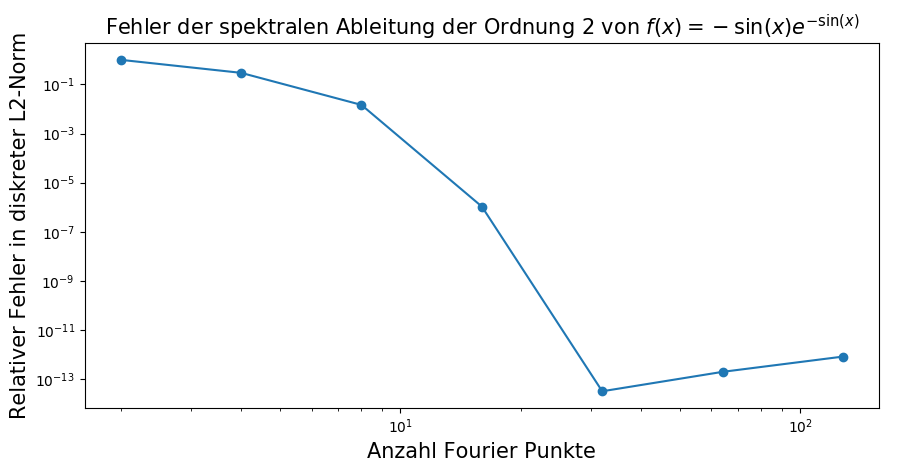
\includegraphics[width=0.9\linewidth]{Figures/spectral_derivative_error_cont.png}
  \caption{Konvergenz der spektralen Ableitung zweiter Ordnung von $f_1$.}
\end{figure}
\begin{figure}[!htb]
  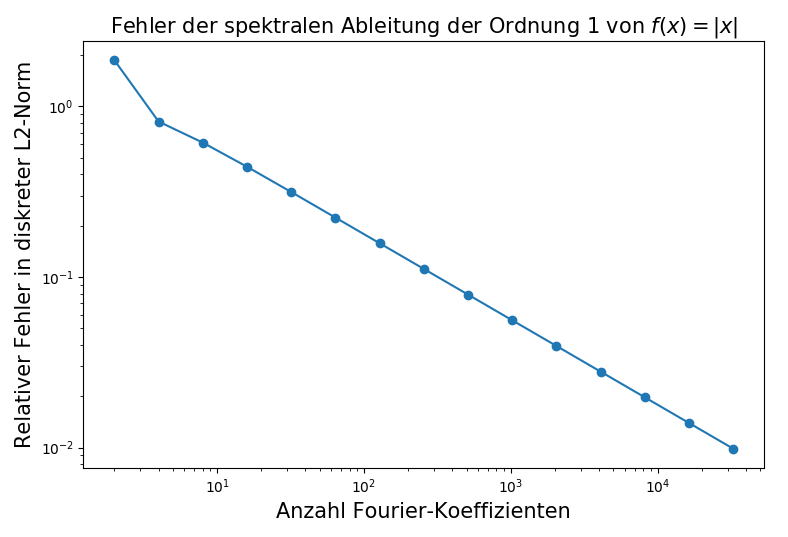
\includegraphics[width=0.9\linewidth]{Figures/spectral_derivative_error_discont.png}
  \caption{Konvergenz der spektralen Ableitung zweiter Ordnung von $f_2$.}
\end{figure}
Wir erkennen, dass die analytische Funktion $f_1$ eine exponentielle Konvergenz aufweist und bereits für $N=64$ Punkte im Bereich der Maschinengenauigkeit liegt. Rechenfehler sorgen bei $N>64$ für eine Aufsummierung von kleinen Überschwingungen und einen langsam wachsenden Fehler.\\
Die stetige Funktion $f_2$ mit stückweise stetiger nicht-periodischer Ableitung leidet bei der Approximation unter dem Gibbs-Phänomen und deutlich langsamerer Konvergenz.
\end{mathbsp}

Formalisieren wir nun die diskrete Fourier-Transformation, die wir verwenden möchten, um eine Approximation an die Fourier-Koeffizienten zu erhalten.
\begin{mathdef}[Diskrete Fourier-Transformation]
Die lineare Abbildung $\mathcal{F}_N\colon\Complex^N\to\Complex^N$ definiert durch
\[\mathcal{F}_Nz=\fourier{z},\qquad\text{mit}\quad \fourier{z}_k=\sum_{j=0}^{N-1}e^{-2\pi i\frac{jk}{N}}z_j\]
heißt diskrete Fourier-Transformation.
\end{mathdef}
Anstelle die direkte Implementierung von $\mathcal{F}_N$ zu verwenden, welche $\mathcal{O}(N^2)$ Rechenschritte benötigt, werden wir auf die deutlich schnellere Berechnung der Abbildung in $\mathcal{O}(N\log N)$ Schritten zurückgreifen. Diese ist unter dem Namen \emph{Fast-Fourier-Transformation} (FFT) bekannt. Da diese auf der Annahme $N=2^p$ für ein $p\in\N$ basiert, werden wir in Zukunft nur noch solche Approximationen verwenden. Dies ist wichtig, um eine optimal schnelle Berechnung der Lösung der KGG zu gewährleisten. Ist $N$ keine Potenz von 2, so runden FFT-Bibliotheken $N$ üblicherweise auf die nächsthöhere Potenz von 2 und man muss eine potentiell erhöhte Rechenzeit in Kauf nehmen.\\
Ohne Beweis gilt $\mathcal{F}_N\overline{\mathcal{F}}_N=NI$ und somit hat die inverse Fourier-Transformation beinahe die selbe Gestalt wie die Fourier-Transformation selbst und kann ebenso schnell berechnet werden.\\
Im Folgenden nehmen wir an, die Fourier-Approximation (\ref{eqn:fourier_approx}) von $u$ sei exakt und berechnen für den $j$-ten Punkt $x_j$ der Diskretisierung:
\begin{equation}
\label{eqn:laplace_approxu}
\Laplace u(t,x_j)=\sum_{k\in\mathcal{J}_N}\fourier{u}_k(t)\partial^2_x e^{ikx_j}=\sum_{k\in\mathcal{J}_N}-k^2\fourier{u}_k(t)e^{ikx_j}
\end{equation}
Dabei ist wegen $d=1$ der Laplace-Operator $\Laplace$ darstellbar als $\Laplace=\partial^2_x$.\\
Betrachten wir nun $(\partial^2_x u(t,x_j))_{j=0,\dots,N-1}$ für den Vektor $u_N(t)=(u(t,x_j))_{j=0,\dots,N-1}$ so gilt
\[(\partial^2_x u(t,x_j))_{j=0,\dots,N-1}\approx \mathcal{F}_N^{-1}\left(\big(-k^2\big)_{k\in\mathcal{J}_N}\odot\mathcal{F}_Nu_N(t)\right)\]
wobei $\odot$ die komponentenweise Multiplikation der Vektoren bezeichnet.\\
Damit erhalten wir für $\beta_N=(\beta(x_j))_{j=0,\dots,N-1}$ die im Ort diskretisierte KGG
\begin{equation}
\label{eqn:kgg_discretespace}
\dtt{u}_N(t)=\alpha \mathcal{F}_N^{-1}\left(\big(-k^2\big)_{k\in\mathcal{J}_N}\odot\mathcal{F}_Nu(t)_N\right) -\beta_N\odot u_N(t)
\end{equation}
Diese werden wir nun in ein System erster Ordnung umschreiben, um anschließend ein Splitting darauf anzuwenden. 

Es gilt für $t>0$, $v_N(t)\coloneqq \dt u_N(t)$ und ein Gewicht $w\in [0,1]$ die zu (\ref{eqn:kgg_discretespace}) äquivalente Darstellung
\begin{align}
\label{eqn:kgg_discrete_first_order_part1}
\dt{\begin{pmatrix}u_N\\v_N\end{pmatrix}}(t)&=
\begin{pmatrix}0 & wI_N\\ \alpha\mathcal{F}_N^{-1}\left(\big(-k^2\big)_{k\in\mathcal{J}_N}\odot\mathcal{F}_N (\cdot )\right) & 0\end{pmatrix}
\begin{pmatrix}u_N\\v_N\end{pmatrix}(t)\\
\label{eqn:kgg_discrete_first_order_part2}
&\quad+\begin{pmatrix}0 & (1-w)I_N\\ -\diag({\beta_N}) & 0\end{pmatrix}
\begin{pmatrix}u_N\\v_N\end{pmatrix}(t).
\end{align}
\subsubsection*{Numerischer Fluss des ersten Teils}
Zuerst betrachten wir den ersten Teil der im Ort diskretisierten KGG (\ref{eqn:kgg_discrete_first_order_part1}) und schreiben diesen für $\fourier{u}_N=\mathcal{F}_Nu_N$ und $\fourier{v}_N=\mathcal{F}_Nv_N$ als
\begin{align*}
\dt{\begin{pmatrix}u_N\\v_N\end{pmatrix}}(t)&=
\begin{pmatrix}0 & wI_N\\ \alpha\mathcal{F}_N^{-1}\left(\big(-k^2\big)_{k\in\mathcal{J}_N}\odot\mathcal{F}_N (\cdot )\right) & 0\end{pmatrix}
\begin{pmatrix}u_N\\v_N\end{pmatrix}(t)\\
\equivalent 
\dt{\begin{pmatrix}\fourier{u}_N\\\fourier{v}_N\end{pmatrix}}(t)&=
\begin{pmatrix}0 & wI_N\\ \alpha\diag\big(-k^2\big)_{k\in\mathcal{J}_N} & 0\end{pmatrix}
\begin{pmatrix}\fourier{u}_N\\\fourier{v}_N\end{pmatrix}(t).
\end{align*}
Damit haben wir nun ein System gewöhnlicher Differentialgleichungen der Größe $2N$ im Fourierraum, welches wir explizit über die Matrixexponentialfunktion lösen können:
\[\begin{pmatrix}\fourier{u}_N\\\fourier{v}_N\end{pmatrix}(t)=\exp\underbrace{\left(t\begin{pmatrix}0 & wI_N\\ \alpha\diag\big(-k^2\big)_{k\in\mathcal{J}_N} & 0\end{pmatrix}\right)}_{=M}
\begin{pmatrix}\fourier{u}_N\\\fourier{v}_N\end{pmatrix}(0)\]
Die Blockmatrix $M$ lässt sich in eine äquivalente Blockdiagonalmatrix umformen, indem zueinander gehörende Einträge der $\fourier{u}_N$ und $\fourier{v}_N$ nebeneinander getauscht werden. Konkret bedeutet dies, dass die $i$-te Komponente des Vektors $\fourier{u}_N$ neben die $i$-te Komponente des Vektors $\fourier{v}_N$ getauscht wird. Die Matrixexponentialfunktion von $M$ lässt sich dann durch die Matrixexponentialfunktion der $2\times 2$ Blöcke $M_k$ berechnen. 
\[\exp(M_k)=\exp\begin{pmatrix}0 & wt\\ -\alpha k^2t & 0\end{pmatrix}=
\begin{pmatrix}\cos(t\sqrt{\alpha w}|k|) & \sinc(t\sqrt{\alpha w}|k|)tw\\-\sinc(t\sqrt{\alpha w}|k|)\alpha |k|^2t & \cos(t\sqrt{\alpha w}|k|)\end{pmatrix}\]
Wir fassen nun die Ergebnisse zum numerischen Fluss des ersten Teil des Splittings (\ref{eqn:kgg_discrete_first_order_part1}) zusammen.\\
Seien $g$ und $h$ die Anfangswerte, so gilt $\fourier{u}_N(0)=\mathcal{F}_Ng$ und $\fourier{v}_N(0)=\mathcal{F}_Nh$. Die Lösung an den Stellen $x_j=-\pi+2\pi\frac{j}{N}\in [-\pi,\pi)$ für $j=0,\dots,N-1$ lässt sich darstellen als
\begin{align*}
u(t,x_j)&=\left(\mathcal{F}_N^{-1}\left[\mathcal{F}_Ng\odot \big(\cos(t\sqrt{\alpha w}|k|)\big)_{k\in\mathcal{J}_N} + \mathcal{F}_Nh\odot \big(\sinc(t\sqrt{\alpha w}|k|)tw\big)_{k\in\mathcal{J}_N}\right]\right)_j\\
\partialdt{u}(t,x_j)&=\left(\mathcal{F}_N^{-1}\left[\mathcal{F}_Ng \odot \big(-\sinc(t\sqrt{\alpha w}|k|)\alpha|k|^2t\big)_{k\in\mathcal{J}_N}+\mathcal{F}_Nh\odot \big(\cos(t\sqrt{\alpha w}|k|)\big)_{k\in\mathcal{J}_N}\right]\right)_j
\end{align*}
Man beachte, dass die Sortierung der Fourier-Koeffizienten in verschiedenen Programmiersprachen verschiedenen Notationen folgt und entsprechend die Indizierung angepasst werden muss. Beispielsweise gilt für die Python3 Bibliothek \emph{numpy} durch die entsprechende Funktion \emph{numpy.fft.fftfreq(8)*8} die Konvention
\[\mathcal{J}_8=\left( 0,  1,  2,  3, -4, -3, -2, -1\right)\]
wobei Matlab die ähnliche Konvention
\[\mathcal{J}_8=\left( 0,  1,  2,  3, 4, -3, -2, -1\right)\]
verwendet.\\[0.3cm]
Obige Erläuterungen gelten für eine räumliche Dimension ($d=1$). Will man nun den Ansatz auf mehrere Dimensionen erweitern, so erhält man ein sehr ähnliches Ergebnis.
Führt man die Fourier-Transformation in jeder Dimension durch, so ergibt sich für $d=2$ die Approximation
\[u(t,x)\approx\sum_{k_1\in\mathcal{J}_N}\fourier{u}_{k_1}(t,x_2)e^{ik_1x_1}=\sum_{k_1\in\mathcal{J}_N}\sum_{k_2\in\mathcal{J}_N}\fourier{u}_{k_1,k_2}(t)e^{i(k_1x_1+k_xx_2)}.\]
Die Funktion $\fourier{u}_{k_1}$ bezeichnet die Fourier-Koeffizienten für die eindimensionale Fourier-Approximation entlang der Richtung $x_1$. Durch eine wiederholte Fourier"=Approximation dieser Funktion erhalten wir die zweidimensionale Fourier-Approximation mit den Fourier-Koeffizienten $\fourier{u}_{k_1,k_2}$.\\
Analog zu der Approximation (\ref{eqn:laplace_approxu}) erhält man
\[\Laplace u(t,x)=\sum_{k_1\in\mathcal{J}_N}-k_1^2\fourier{u}_{k_1}(t,x_2) e^{ik_1x_1}=\sum_{k_1,k_2\in\mathcal{J}_N}-(k_1^2+k_2^2)\fourier{u}_{k_1,k_2}(t)e^{i(k_1x_1+k_2x_2)}\]
Das Vorgehen im Mehrdimensionalen unterscheidet sich also nur durch eine aufwändigere Indizierung, ist jedoch im Kern dieselbe. Ersetzt man in obigen Ausführungen für $d=1$ sämtliche $|k|$ durch \[\norm{k}_2=\sqrt{k_1^2+\dots+k_d^2}\]so erhält man, bei passender Indizierung der diskreten Fourier-Approximation, eine Darstellung der Lösung für beliebige Dimensionen $d\in\N$.
\subsubsection*{Method of lines für den zweiten Teil des Splittings}
Einen numerischen Löser für den zweiten Teil (\ref{eqn:kgg_discrete_first_order_part1}) der im Ort diskretisierten KGG erhält man auf ähnliche Weise. Wir suchen für $t>0$, $\beta(x)>0$ und ein Gewicht $\tilde{w}=1-w\in [0,1]$ die Lösung der Differentialgleichung
\begin{equation*}
\dt{\begin{pmatrix}u_N\\v_N\end{pmatrix}}(t)=
\begin{pmatrix}0 & \tilde{w}I_N\\ -\diag({\beta_N}) & 0\end{pmatrix}
\begin{pmatrix}u_N\\v_N\end{pmatrix}(t)
\end{equation*}
Die Struktur der Differentialgleichung zeigt, dass sich ihre Lösung ebenfalls mithilfe der Matrixexponentialfunktion darstellen lässt. Die Matrixexponentialfunktion der Blockmatrix ist wiederum durch nebeneinander Sortieren der $i$-ten Komponenten der Vektoren $u_N$ und $v_N$ äquivalent zu einer Blockdiagonalmatrix mit $2\times 2$ Blöcken auf der Diagonalen. Für diese gelten:
\[\exp\begin{pmatrix}0 & \tilde{w}t\\ -t\beta(x_j) & 0\end{pmatrix}=
\begin{pmatrix}\cos(t\sqrt{\beta(x_j)\tilde{w}}) & \sinc(t\sqrt{\beta(x_j)\tilde{w}})\tilde{w}t\\
-\sinc(t\sqrt{\beta(x_j)\tilde{w}})\beta(x_j)t & \cos(t\sqrt{\beta(x_j)\tilde{w}})\end{pmatrix}\]
Daraus erhalten wir zu den Anfangswerten $g$ und $h$ für festes $x\in \Torus^d$ die explizite Lösung des zweiten Teil des Splittings durch
\[\begin{pmatrix}u\\v\end{pmatrix}(t,x)=
\begin{pmatrix}\cos(t\sqrt{\beta(x)\tilde{w}}) & \sinc(t\sqrt{\beta(x)\tilde{w}})\tilde{w}t\\
-\sinc(t\sqrt{\beta(x)\tilde{w}})\beta(x)t & \cos(t\sqrt{\beta(x)\tilde{w}})\end{pmatrix}
\begin{pmatrix}g\\h\end{pmatrix}(x)\]
Wir benötigen im Gegensatz zum ersten Teil keine feste Ortsdiskretisierung und bekommen sogar eine exakte Lösung des Teilproblems. Da die Punkte für die verschiedenen Teile des Splittings identisch sein müssen, sind wir jedoch durch die Anforderung festgelegt, die die Fourier-Approximation an die Punkte stellt.\\
Mithilfe der \emph{method of lines}, d.h. punktweiser Auswertung der Lösung für alle benötigten $x$, bekommt man schlussendlich eine numerische Lösung.
\subsubsection*{Konkretisierung des Algorithmus}
Wir haben nun zwei separate Einschrittverfahren, die zusammen mit dem Strang-Splitting Framework einen guten Löser für die KGG ergeben. Dieses Lösungsverfahren ist für $d=1$ schematisch als Algorithmus \ref{alg:kgg_solver} dargestellt.
\begin{algorithm}[ht]
    \caption{Strang-Splitting für KGG}
    \label{alg:kgg_solver}
    \begin{algorithmic}[1] % The number tells where the line numbering should start
    	\Function{Fast\_Strang}{$N,u_0,v_0,\alpha,\beta,w,\tau,T$}
    		\State $x_N\gets (-\pi+\frac{2\pi j}{N})_{j=0,\dots,N-1}^T$
            \State $g,h\gets u_0(x_N), v_0(x_N)$
            \State $g,h\gets \text{First\_Part\_Solver}(N, g, h, \alpha, w, \frac{\tau}{2})$
            \State $g,h\gets \text{Second\_Part\_Solver}(x_N, g, h, \beta, 1-w, \tau)$
            \For{$i=1,\dots,\frac{T}{\tau}-1$} \Comment{Annahme: $\frac{T}{\tau}\in\N$} 
            	\State $g,h\gets \text{First\_Part\_Solver}(N, g, h, \alpha, w, \tau)$
            	\State $g,h\gets \text{Second\_Part\_Solver}(x_N, g, h, \beta, 1-w, \tau)$
            \EndFor
            \State $u_1,v_1\gets \text{First\_Part\_Solver}(N, g, h, \alpha, w, \frac{\tau}{2})$            
            \State \textbf{return} $u_1$ \Comment{Approximation an $u(T,x_N)$}
    	\EndFunction
        \Function{Strang\_Step\_KGG}{$N,u_0,v_0,\alpha,\beta,w,\tau$} 
            \State $x_N\gets (-\pi+\frac{2\pi j}{N})_{j=0,\dots,N-1}^T$
            \State $g,h\gets u_0(x_N), v_0(x_N)$
            \State $g,h\gets \text{First\_Part\_Solver}(N, g, h, \alpha, w, \frac{\tau}{2})$
            \State $g,h\gets \text{Second\_Part\_Solver}(x_N, g, h, \beta, 1-w, \tau)$
            \State $u_1,v_1\gets \text{First\_Part\_Solver}(N, g, h, \alpha, w, \frac{\tau}{2})$
            \State \textbf{return} $u_1, v_1$\Comment{Approximation an $u(\tau,x_N)$ und $\dt{u}(\tau,x_N)$}
        \EndFunction
        
        \Function{First\_Part\_Solver}{$N,g,h,\alpha,w,\tau$} 
        	\State Indexmenge $\mathcal{J}_N$ für Fourierkoeffizienten initialisieren
        	\State $\fourier{g}\gets \mathcal{F}_Ng$
        	\State $\fourier{h}\gets \mathcal{F}_Nh$
        	\State $c\gets \big(\cos(\tau\sqrt{\alpha w}|k|)\big)_{k\in\mathcal{J}_N}$
        	\State $s_1\gets \big(\sinc(\tau\sqrt{\alpha w}|k|)\tau w\big)_{k\in\mathcal{J}_N}$
        	\State $s_2\gets \big(-\sinc(\tau\sqrt{\alpha w}|k|)\alpha|k|^2\tau\big)_{k\in\mathcal{J}_N}$
            \State \textbf{return} $\mathcal{F}_N^{-1}\left(\fourier{g}\odot c+\fourier{h}\odot s_1\right),\quad \mathcal{F}_N^{-1}\left(\fourier{g}\odot s_2+\fourier{h}\odot c\right)$
        \EndFunction
        \Function{Second\_Part\_Solver}{$x_N,g,h,\beta,\tilde{w},\tau$} 
        	\State $\beta_N\gets\beta(x_N)$
        	\State $c\gets \cos(\tau\sqrt{\beta_N}\sqrt{\tilde{w}})$
        	\State $s_1\gets \sinc(\tau\sqrt{\beta_N}\sqrt{\tilde{w}})\tilde{w}\tau$
        	\State $s_2\gets -\sinc(\tau\sqrt{\beta_N}\sqrt{\tilde{w}})\beta_N\tau$
        	\State \textbf{return} $g\odot c+h\odot s_1,\quad g\odot s_2+h\odot c$
        \EndFunction
    \end{algorithmic}
\end{algorithm}

Dabei ist die Wahl gewisser Parameter jedoch noch unklar:
\begin{itemize}
\item Die Anzahl der Fourierpunkte $N$.
\item Das Gewicht $w\in[0,1]$ für die Gewichtung des Splittings. 
\end{itemize}
Um die Zusammenhänge und Probleme besser zu verstehen, werden wir anhand eines Beispiels mit bekannter exakter Lösung verschiedene Kombinationen der Parameter demonstrieren.
\begin{mathbsp}
\label{bsp:trialfrog2}
Sei $c>2$, dann ist
\begin{align*}
u(t,x)&=\frac{\cos(t)}{\sin(x)+c}\\
u_0(x)&=\frac{1}{\sin(x)+c}\\
v_0(x)&\equiv 0\\
\end{align*}
eine Lösung der eindimensionalen KGG (\ref{kgg}) mit $\alpha=c-2$ und $\beta(x)=1+(c-2)\left(\frac{\sin(x)}{\sin(x)+c}+\frac{2\cos^2(x)}{(\sin(x)+c)^2}\right)$. Wir lösen nun die KGG mithilfe verschiedener Splitting-Varianten und beobachten in Abbildung \ref{fig:splitting_convergence}
\begin{itemize}
\item für das Strang-Splitting die erwartete Konvergenz von Ordnung 2.
\item für das Lie-Trotter-Splitting die erwartete Konvergenz von Ordnung 1.
\item für die schnelle Variante des Strang-Splittings (FastStrang), bei der die äußeren Halbschritte kombiniert werden, exakt den gleichen Fehler wie beim Standard Strang-Splitting.
\item für die umgekehrte Variante des Strang-Splittings (ReversedStrang), wo die Reihenfolge der beiden Aufteilungen der Gleichung vertauscht wurde, eine minimale Abweichung von der Standardvariante.
\item ein deutliches Problem: Wird die Zeitschrittweite $\tau$ zu groß, d.h. ist $1.227\tau>\frac{2\pi}{N}=h$, so ist das Verfahren instabil!
\end{itemize}
\begin{figure}[!htb]
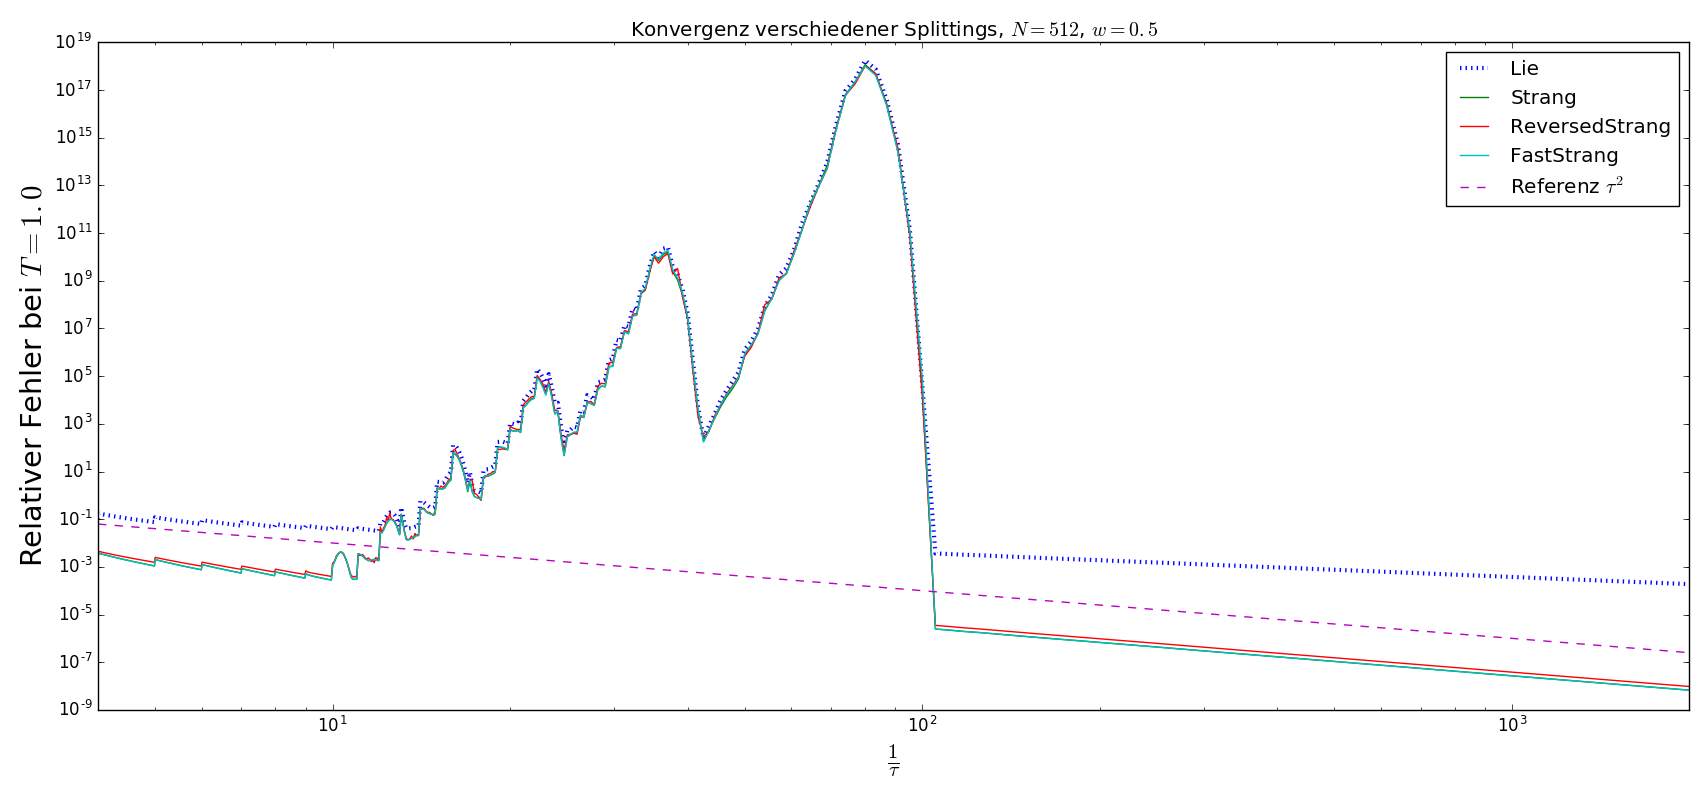
\includegraphics[width=\textwidth]{Figures/splitting_convergence_fix_weight_frog2_cfl.png}
\caption{Konvergenzordnung für verschiedene Splitting-Varianten anhand von Beispiel \ref{bsp:trialfrog2} mit $c=3$, $d=1$, $N=512$, $w=0.5$ zum Zeitpunkt $T=1$.}
\label{fig:splitting_convergence}
\end{figure}
Für die beobachtete Instabilität spielt der Gewichtsfaktor $w$ eine große Rolle. Wäre $w=0$, so entspricht der Löser des ersten Teil des Splittings der Vorschrift
\begin{align*}
u(t,x_N)&=\mathcal{F}_N^{-1}\left(\mathcal{F}_Ng(x_N)\right)=g(x_N)=u(0,x_N)\\
\dt{u}(t,x_N)&=\mathcal{F}_N^{-1}\left(\mathcal{F}_Ng(x_N)\odot \big(-\alpha |k|^2t\big)_{k\in\mathcal{J}_N}\right)+h(x_N)\\
&=t \alpha \mathcal{F}_N^{-1}\left(\mathcal{F}_N\odot \big(-|k|^2\big)_{k\in\mathcal{J}_N}\right)+h(x_N)\\
&=t\alpha \Laplace_N g(x_N)+h(x_N)\\
&\approx t\dtt{u}(0,x_N)+\dt{u}(0,x_N)
\end{align*}
Somit wird in diesem Randfall nur die erste Ableitung geändert und dieses Update entspricht einem expliziten Eulerschritt für die erste Ableitung. Das Splittingverfahren ist dann äquivalent zu einem sogenannten Leapfrog-Verfahren, welches schneller zu berechnen ist, da eine Anwendung von $\mathcal{F}_N^{-1}$ entfällt. Wir erhalten für die Stabilität eine \emph{Courant-Friedrichs-Lewy-Bedingung} (CFL-Bedingung) der Form $\tilde{c}\tau\le h=\frac{2\pi}{N}$. Im Fall $k=0$ entspricht die CFL-Zahl $\tilde{c}$ der CFL-Zahl des expliziten Eulers.\\[0.3cm]
Wir beobachten an Abbildung \ref{fig:splitting_cfl}, dass die CFL-Zahl abhängig von $w$ ist und für $w=1$ ein Minimum annimmt. Die Kurven für verschiedene $N$ weichen dabei voneinander ab, da die Schätzung des kleinsten Zeitpunkts, für welchen die Berechnung instabil ist, heuristisch ist. Wir definieren die Berechnung als instabil, wenn die absolute Steigung im Ordnungsplot kleiner als 1 oder größer als 3 ist oder der beobachtete relative Fehler größer als 1 ist. Diese Instabilitätseffekte beobachtet man für $w\to 1$ erst für große $\tau$, die bei $T=1$ nur sehr wenigen Splittingschritten entsprechen.
\begin{figure}[!htb]
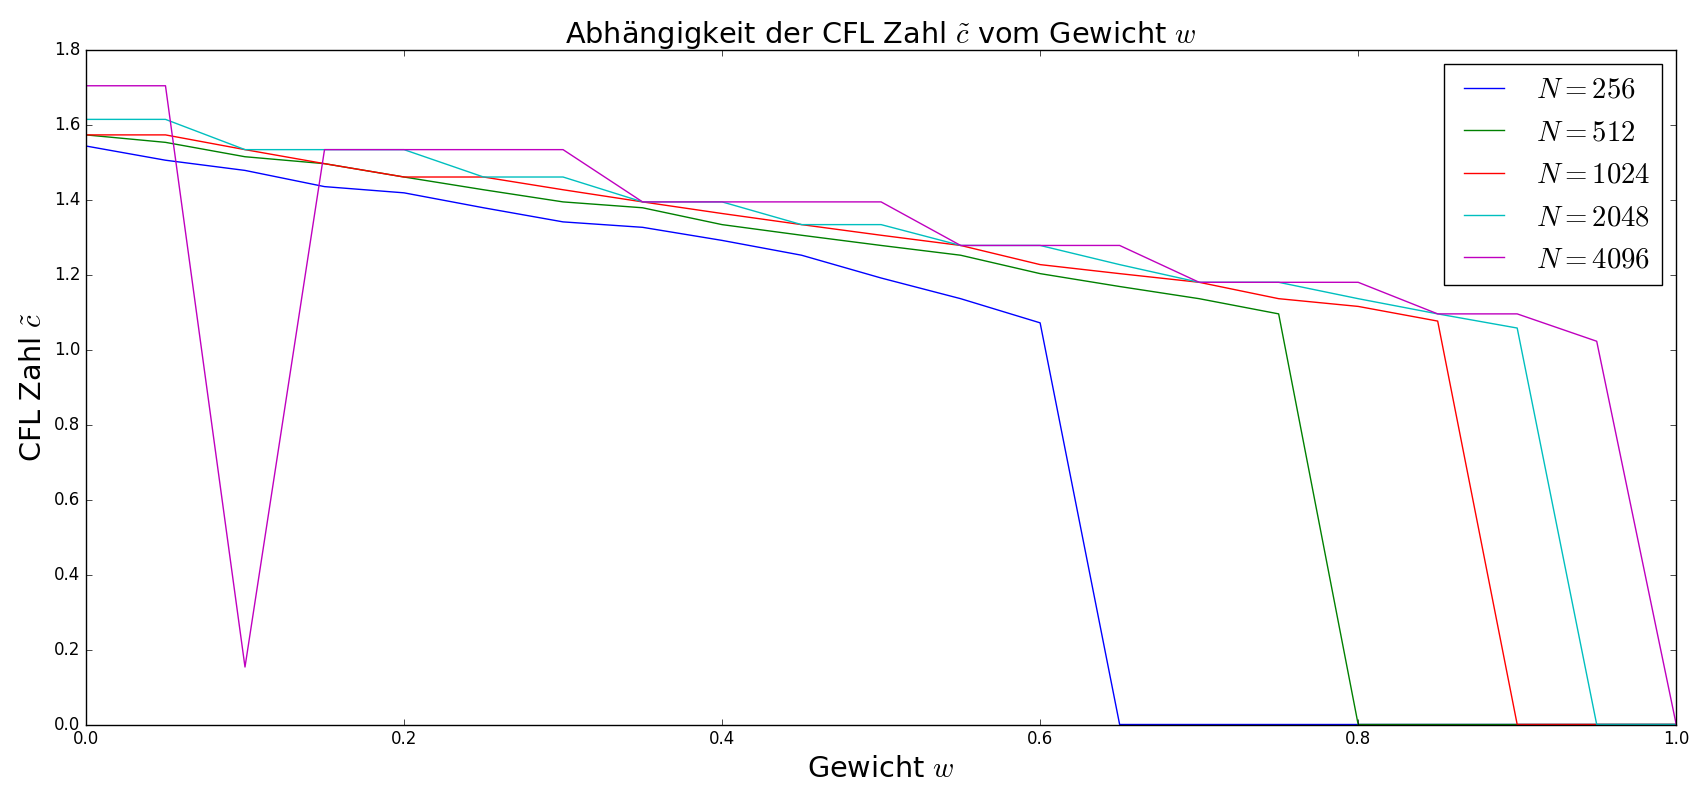
\includegraphics[width=\textwidth]{Figures/cfl_estimations_frog2.png}
\caption{Abhängigkeit der CFL-Zahl anhand von Beispiel \ref{bsp:trialfrog2} mit $c=3$ und $d=1$ zum Zeitpunkt $T=1$.}
\label{fig:splitting_cfl}
\end{figure}
\\[0.3cm]
Wie man an Abbildung \ref{fig:splitting_convergence_w1} erkennt, verhält sich für $w=1$ die Gleichung am stabilsten und kann auch für große Zeitschrittweiten sinnvoll gelöst werden. Dies wird eine große Motivation dafür sein, das Gewicht $w=1$ zu wählen.

\begin{figure}[!htb]
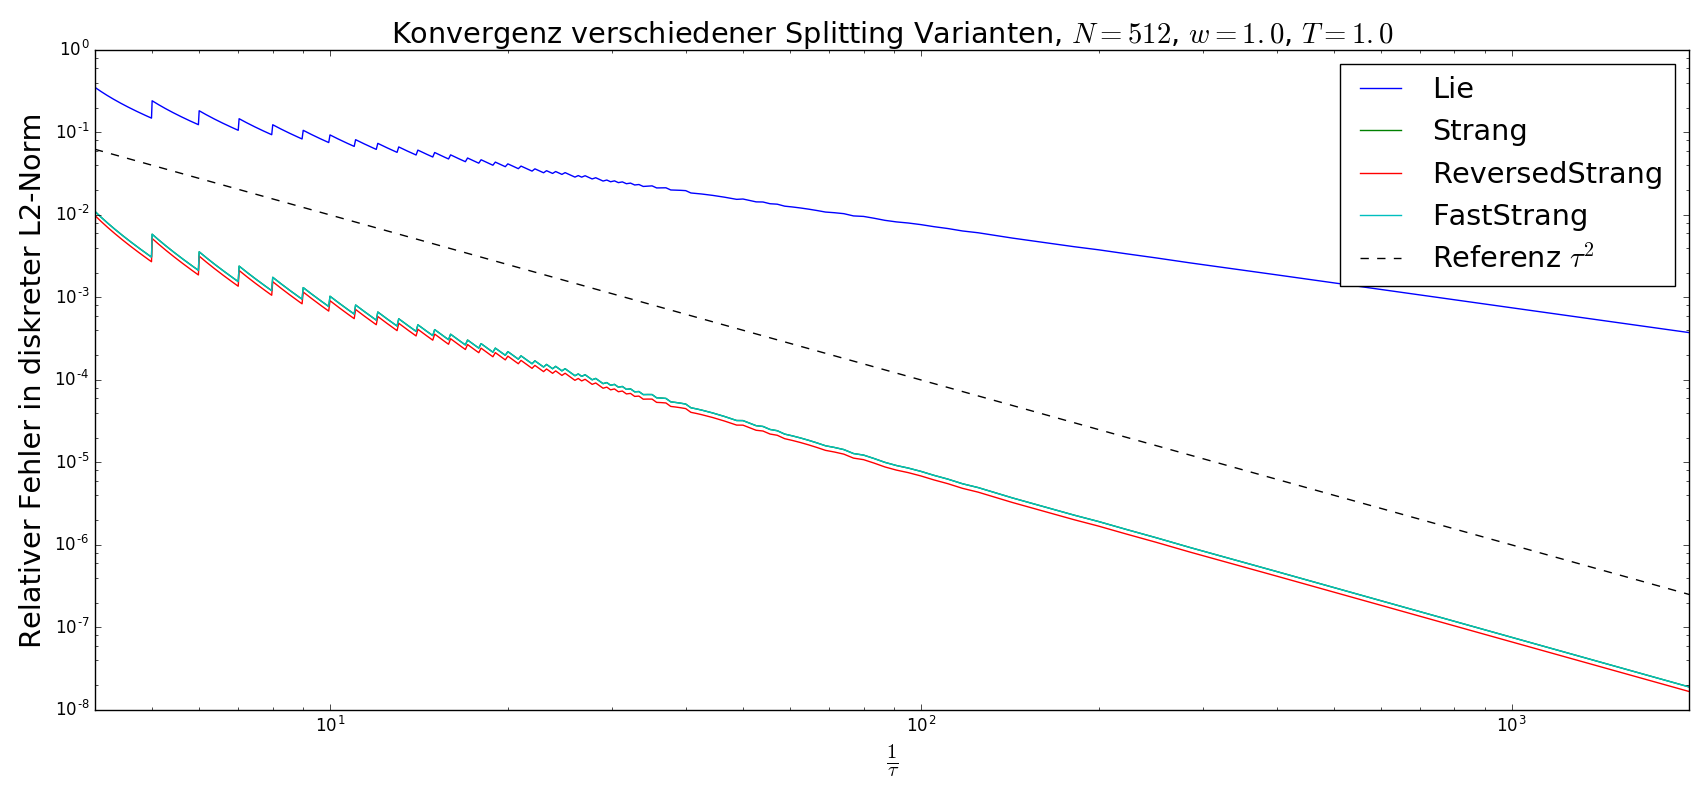
\includegraphics[width=\textwidth]{Figures/splitting_convergence_fix_weight_frog2_cfl_corrected.png}
\caption{Konvergenzordnung für verschiedene Splitting-Varianten anhand von Beispiel \ref{bsp:trialfrog2} mit $c=3$, $d=1$, $N=512$, $w=1$ zum Zeitpunkt $T=1$.}
\label{fig:splitting_convergence_w1}
\end{figure}
Zuletzt sei aber erwähnt, dass die Wahl $w=1$ aus Sicht des minimalen Fehlers selten optimal ist. An Abbildung \ref{fig:splitting_dependence_on_weight} erkennen wir für verschiedene bekannte Lösungen der KGG, dass das Minimum des Fehlers in Abhängigkeit vom Gewicht $w$ sowohl an beiden Rändern, als auch als lokales Minimum auftreten kann. Das genaue Minimum zu bestimmen und dies mit der CFL-Zahl zu kombinieren, um das optimale $w$ zu wählen, kann ein möglicher Ansatz zur Verbesserung des Algorithmus sein. Wir werden dies jedoch nicht weiter verfolgen und uns in den meisten Fällen auf $w=1$ beschränken, da eine Verbesserung des Fehlers dann mit einer Verringerung der Schrittweite $\tau$ besser kontrollierbar ist.
\begin{figure}[!htb]
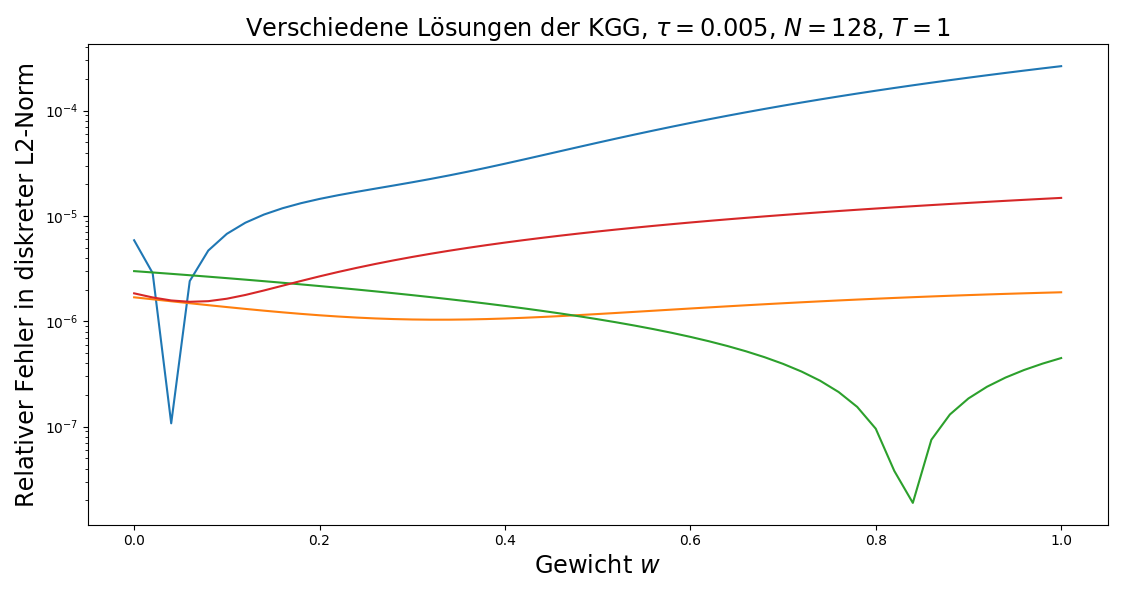
\includegraphics[width=\textwidth]{Figures/splitting_error_over_weights.png}
\caption{Verschiedene Beispiele von bekannten Lösungen der KGG gelöst mit FastStrang. Der Fehler wird dabei in Abhängigkeit des Gewichts $w$ verglichen.}
\label{fig:splitting_dependence_on_weight}
\end{figure}
\end{mathbsp}

\section{Stochastische Modellierung}
In diesem Abschnitt werden wir erläutern, wie man stochastische Einflüsse, insbesondere zufällige Koeffizienten $\alpha$ und $\beta$, auf die KGG darstellen kann. Die Modellierung, die hier gezeigt wird ist dabei viel allgemeiner gehalten, als wir sie später verwenden werden. Dies entspricht dem praktischen Vorgehen in den Anwendungen und motiviert die Verwendung von stochastischer Modellierung bei Differentialgleichungen. In unserem Fall werden wir uns auf Zufallsvektoren mit bekannten Komponentenverteilungen beschränken.
\subsection{Grundbegriffe}
Wir geben keine Einführung in die klassische Wahrscheinlichkeitstheorie, werden aber die relevanten Begriffe und Definitionen an dieser Stelle kurz wiederholen. Es sei angemerkt, dass neben den vorgestellten stetigen Verteilungen auch diskrete Verteilungen wie die Poisson-Verteilung existieren und sich durch dieselbe Theorie beschreiben lassen. Um die Notation zu vereinfachen, werden wir jedoch ausschließlich stetige Verteilungen betrachten.

\begin{mathdef}[Wahrscheinlichkeitsraum]
Ein Wahrscheinlichkeitsraum $(\Omega,\mathcal{F},P)$ ist ein Tripel bestehend aus 
\begin{itemize}
\item der abzählbaren nichtleeren Ergebnismenge $\Omega$
\item der $\sigma$-Algebra der Ereignisse $\mathcal{F}$ über der Grundmenge $\Omega$
\item dem Wahrscheinlichkeitsmaß $P\colon\mathcal{F}\to [0,1]$
\end{itemize}
\end{mathdef}

\begin{mathdef}[Verteilungsfunktion]
Die Verteilungsfunktion $F_Y$ der Zufallsvariablen $Y\colon\Omega\to\R$ ist definiert durch
\[F_Y(y)\coloneqq P(Y\le y)=P(\left\lbrace \omega\in\Omega |\: Y(\omega)\le y\right\rbrace),\quad y\in\R\]
\end{mathdef}
\begin{mathdef}[Dichte einer Verteilung]
Existiert zu der Verteilungsfunktion $F_Y$ der Zufallsvariablen $Y\colon\R\to\R$ eine Funktion $\rho_Y\colon\R\to\R_{\ge 0}$ mit
\[F_Y(y)=\int_{-\infty}^y\rho_Y(z)dz,\quad y\in\R\]
so nennen wir diese die Dichte von $F_Y$.\\
Für stetige Zufallsvariablen folgt die Existenz aus dem Satz von Radon-Nikodým.
\end{mathdef}
\begin{mathdef}[Stochastische Unabhängigkeit]
Ist $(\Omega,\mathcal{F},P)$ ein Wahrscheinlichkeitsraum und $Y_1, Y_2\colon \Omega\to\R$ zwei reelle Zufallsvariablen, so nennt man $Y_1$ und $Y_2$ (stochastisch) unabhängig genau dann wenn
\[P(Y_1\in B_1,Y_2\in B_2)=P(Y_1\in B_1)P(Y_2\in B_2)\]
für alle $B_1,B_2\in \mathcal{B}(\R)$, der Borelschen $\sigma$-Algebra über $\R$.
\end{mathdef}
\begin{mathbsp}
Ist $\mathcal{N}(\mu, \sigma^2)$ die Normalverteilung mit Parametern $\mu\in\R$ und $\sigma^2>0$ so gilt für ihre Dichtefunktion
\[\rho_Y(y)=\frac{1}{\sqrt{2\pi\sigma^2}}e^{-\frac{(y-\mu)^2}{2\sigma^2}},\quad y\in\R\,.\]
Ist $\mathcal{U}(a,b)$ die Gleichverteilung auf $(a,b)$ so gilt für ihre Dichtefunktion
\[\rho_Y(y)=\begin{cases}\frac{1}{b-a},\quad &y\in (a,b)\\ 0, \quad &\text{sonst}\,. \end{cases}\]
\end{mathbsp}
Folgende Definitionen werden die später hauptsächlich untersuchten Eigenschaften von zufallsabhängigen Größen darstellen.
\begin{mathdef}[Erwartungswert und Varianz]
Ist $Y\colon\R\to\R$ eine reelle Zufallsvariable mit Dichte $\rho_Y$ so definieren wir den Erwartungswert von $Y$ als
\[\mu_Y=\E[Y]=\int_{-\infty}^\infty y\rho_Y(y)dy\]
und die Varianz von $Y$ als 
\[\sigma_Y^2=\text{var}(Y)=\int_{-\infty}^\infty (y-\mu_Y)^2\rho_Y(y)dy=\E[Y^2]-\E[Y]^2\]
\end{mathdef}
Ohne Beweis präsentieren wir die Inversionsmethode. Diese ist nützlich um aus Zufallsvariablen einer bestimmten Verteilung Zufallsvariablen einer anderen Verteilung zu gewinnen. In der Numerik ist dies ist essentiell für die Erzeugung von Pseudozufallszahlen von beliebigen Verteilungen. Die Methode ist aber auch wichtig für die "`stochastische Normierung"' von verschiedenen Zufallsvariablen zu einem gemeinsamen Wahrscheinlichkeitsraum, auf dem dann Erwartungswerte berechnet werden können.
\begin{maththeorem}[Inversionsmethode]
\label{thinversionsmethode}
Ist $Y$ eine reelle Zufallsvariable mit Verteilungsfunktion $F_Y$, so definieren wir deren Quantilfunktion als
\[F_Y^{-1}(p)\coloneqq \inf\lbrace y\in\R |\: F_Y(y)\ge p\rbrace,\quad p\in\R\]
Dann gilt
\begin{itemize}
\item $z\le F_Y(y)\iff F_Y^{-1}(z)\le y$\\
\item Falls $Z$ gleichverteilt in $(0,1)$ ist, dann hat $F_Y^{-1}(Z)$ die Verteilungsfunktion $F_Y$. 
\end{itemize}
\end{maththeorem}
Der auch \emph{Gesetz der großen Zahlen} genannte Zentrale Grenzwertsatz bildet die Grundlage für das erste Verfahren zur Berechnung von Erwartungswert und Varianz.
\begin{maththeorem}[Zentraler Grenzwertsatz]
\label{thzentralgrenzwert}
Seien $Y_1,Y_2,\dots,Y_n$ unabhängige und identisch verteilte Zufallsvariablen mit $\E[Y_i]=\mu$ und $\text{var}(Y_i)=\sigma^2<\infty$ Der Mittelwert sei definiert als
\[\overline{Y}\coloneqq \frac{1}{n}\sum_{i=1}^nY_i\]
und skaliert durch
\[Z_n=\sqrt{n}\left(\frac{\overline{Y}-\mu}{\sigma}\right)\]
Dann konvergiert für $n\to\infty$ die Verteilungsfunktion von $Z_n$ zu einer $\mathcal{N}(0,1)$ verteilten Verteilungsfunktion.
\end{maththeorem}
\begin{mathdef}[Zufallsvektoren]
Wir nennen $Y=(Y_1,\dots,Y_n)$ einen $n$-dimensionalen Zufallsvektor (häufig auch einfach $n$-dimensionale Zufallsvariable), wenn die Komponenten $Y_1,\dots,Y_n\colon\Omega\to\R$ eindimensionale reelle Zufallsvariablen sind. Sind die Komponenten $Y_i$ stochastisch unabhängig und besitzt jede Komponente $Y_i$ eine Dichte $\rho_{Y_i}$, so gilt die wichtige Darstellung der gemeinsamen Dichtefunktion $\rho_Y$
\[\rho_Y=\prod_{i=1}^n \rho_{Y_i}\]
und die Verteilungsfunktion lässt sich darstellen als
\[F_Y(y_1,\dots,y_n)=\int_{-\infty}^{y_1}\dots\int_{-\infty}^{y_n}\rho_Y(z_1,\dots,z_n)dy_1\dots dy_n\]
\end{mathdef}

\subsection{Endliche Parametrisierung}
\label{secfiniteparam}
Dieser Abschnitt beschäftigt sich mit der Frage, wie man, ausgehend von einem potentiell unendlich-dimensionalen Wahrscheinlichkeitsraum, eine endliche Approximation desselben erhalten kann. Diese Approximation soll in der Form von $n$ stochastisch unabhängigen Zufallsvariablen vorliegen, welche zu einem $n$-dimensionalen Zufallsvektor zusammen gefasst werden. Die Bedingung der Unabhängigkeit ist dabei theoretisch zwar wenig einschränkend, aber eine sehr wichtige Grundlage für viele praktische numerische Verfahren.\\
Im Fall unserer stochastischer Klein-Gordon-Gleichung steckt die Zufallsabhängigkeit direkt in den Modellparametern $\alpha$ und $\beta$ und in den Anfangswerten. Auch wenn die Zufallsabhängigkeit wie in diesem Fall direkt im Modell gegeben ist, muss für numerische Lösungsverfahren eine Charakterisierung derselben durch endlich viele unabhängige Zufallsvariablen mit bekannter Verteilung sicher gestellt werden.\\
Wir werden später stets davon ausgehen, dass bereits eine endliche Parametrisierung durch unabhängige Zufallsvariablen mit bekannter Verteilung vorliegt. Der Vollständigkeit halber seien hier kurz Methoden genannt, um das Parametrisierungsproblem zu lösen. Man beachte jedoch, dass einige der Methoden numerisch nicht umsetzbar oder ad-hoc-Lösungen sind, die spezielle Annahmen benötigen. Dieser Abschnitt wurde aus \autocite[Kapitel 4.1+4.2]{dongbinxiu2010} übernommen, wo auch Visualisierungen und kleine Beispiele zu finden sind.

\subsubsection{Unabhängigkeit von endlich vielen Parametern}
Wenn die Zufallsabhängigkeit des Modells bereits durch endlich viele Modellparameter vorliegt, ist die Parameterisierung auf natürliche Art gegeben. Wichtig ist dann, die unabhängigen Parameter zu identifizieren bzw. die Abhängigkeit zu konkretisieren.\\
Für normalverteilte Parameter ist dies auch auf einfache Weise möglich:
\begin{maththeorem}
\label{thgaussunabhg}
Sei $Z\sim\mathcal{N}(0,I_n)$, wobei $I_n$ die n-dimensionale Einheitsmatrix ist, ein unkorrelierter Zufallsvektor. Für die Gaussverteilung ist Unkorreliertheit äquivalent zu Unabhängigkeit und die Komponenten von $Z$ sind somit unabhängig. Sei $A\in\R^{n\times n}$ eine reguläre untere Dreiecksmatrix. Dann gilt:
\[Y\coloneqq AZ\sim\mathcal{N}(0,AA^T)\]
Da die Kovarianzmatrix $C\in\R^{n\times n}$ eines $\mathcal{N}(0,C)$ verteilten Zufallsvektors $Y$ symmetrisch und positiv definit ist, existiert die Cholesky-Zerlegung $C=AA^T$ mit einer regulären unteren Dreicksmatrix $A$. Folglich kann $Y$ durch stochastisch unabhängige Parameter $Z_1,\dots,Z_n$ dargestellt werden.
\end{maththeorem}
Sind die Parameter nicht normalverteilt, so wird das Problem deutlich schwieriger und bis jetzt gibt es keine zufriedenstellende numerische Transformation, die entsprechendes zu Satz \ref{thgaussunabhg} leistet. Eine theoretische Möglichkeit bietet sich jedoch über die Rosenblatt-Transformation, welche auf den in der Praxis selten bekannten bedingten Wahrscheinlichkeiten basiert.

\subsubsection{Parametrisierung von Zufallsprozessen}
Häufig sind die Zufallsabhängigkeiten des Modells nur durch Beobachtungen oder Messungen von Zufallsvariablen möglich. Wir schreiben diese als stochastischen Prozess $(Y_t,t\in T)$, wobei $T$ die Indexmenge ist und $Y_t$ die beobachteten Zufallsvariablen. Wir suchen dann eine Transformation $R$, welche die Darstellung $Y_t=R(Z)$ mit Zufallsvektor $Z=(Z_1,\dots,Z_n)$ und unabhängigen Komponenten $Z_i$ erlaubt. Da $T$ potentiell ein unendlich-dimensionaler Raum ist, kann diese Transformation nicht exakt sein und wir suchen nun eine in einem gewissen Sinne bestmögliche Approximation.\\
Die am häufigsten verwendete Technik ist dabei die Karhunen-Loeve-Darstellung.
\begin{mathdef}[Karhunen-Loeve-Darstellung]
Sei $\mu_Y(t)$ der Erwartungswert des Prozesses $Y_t$ am Punkt $t$ und sei $C(t,s)=\text{cov}(Y_t,Y_s)$ die Kovarianzfunktion. Dann ist die Karhunen-Loeve-Darstellung definiert als
\[Y_t(\omega)=\mu_Y(t)+\sum_{i=1}^\infty \sqrt{\lambda_i}\Psi_i(t)Z_i(\omega)\] wobei $\Psi_i$ die orthogonalen Eigenfunktionen und $\lambda_i$ die zugehörigen Eigenwerte des Eigenwertproblems
\[\int_T C(t,s)\Psi_i(s)ds=\lambda_i\Psi_i(t),\quad t\in T\]
sind. Die paarweise unkorrelierten Zufallsvariablen $Z_i(\omega)$ erfüllen
\[\E[Z_i]=0,\quad \E[Z_iZ_j]=\delta_{ij}\]
und sind definiert durch
\[Z_i(\omega)=\frac{1}{\sqrt{\lambda_i}}\int_T (Y_t(\omega)-\mu_Y(t))\Psi_i(t)dt\]
Um eine Approximation zu erhalten wird die Reihe bei einem gewissen Index $n\in\N$ abgebrochen.
\end{mathdef}
Wiederrum erhält man daraus für normalverteilte Prozesse eine endliche Menge von unabhängigen Zufallsvariablen. Für nicht-normalverteilte Prozesse wird häufig dennoch die Karhunen-Loeve-Darstellung verwendet und zusätzlich angenommen, dass die $Z_i$ unabhängig sind. Diese Vorgehensweise ist nicht sehr zufriedenstellend und ein offenes Forschungsproblem.

\subsection{Formulierung der stochastischen Klein-Gordon-Gleichung}
In Analogie zur Klein-Gordon-Gleichung (\ref{kgg}) definieren wir für einen Wahrscheinlichkeitsraum $(\Omega,\mathcal{F},P)$ und $Y\colon\Omega\to\R^N$ die stochastische Klein-Gordon-Gleichung (sKGG) für $y=Y(\omega)$ durch
\begin{align}
\label{skgg}
\dtt{u}(t,x,y)&=\alpha(y) \Laplace u(t,x,y) - \beta(x,\omega)u(t,x,y), \: t>0, \, x\in \Torus^d\\
u(0,x,y)&=u_0(x,y), \: x\in \Torus^d\\
\dt{u}(0,x,y)&=v_0(x,y), \: x\in \Torus^d
\end{align}
Die Lösung \[u(t,x,y)\colon [0,T]\times\Torus^d\times \R^N\to\R\] ist folglich eine zufallsabhängige Größe.\\
Dabei ist die grundlegende Annahme, dass (\ref{skgg}) $P$-fast-sicher wohl gestellt ist, d.h. die Menge an Punkten $\omega$, für welche die partielle Differentialgleichung mit fixem $y=Y(\omega)$ keine eindeutige Lösung besitzt, ist eine Nullmenge bezüglich des Wahrscheinlichkeitmaßes $P$.\\
Wie bereits in Kapitel \ref{secfiniteparam} diskutiert, werden wir stets annehmen, dass die Komponenten $Y_i$ von $Y$ stochastisch unabhängige Zufallsvariablen mit bekannter Verteilung sind.
\begin{mathbsp}
\label{bsp:trial1}
Sei $Y=(Y_1)$ eine eindimensionale und in $(2,3)$ gleichverteilte Zufallsvariable. Dann gilt für $t>0$, $d\in\N$, $x=(x_1,\dots$, $x_d)\in\Torus^d$, $\hat{x}\coloneqq \sum_{i=1}^d x_i$, $y=Y(\omega)$ und Anfangswerten $u_0(x,y)=2\sin(\hat{x})$, $v_0(x,y)\equiv 0$:
\begin{equation*}
u(t,x,y)=2\cos(ty)\sin(\hat{x})
\end{equation*}
löst die stochastische KGG (\ref{skgg}) für $\alpha(y)=\frac{y}{d}$ und $\beta(x,y)=y^2-y$. Diese Parameter und Anfangswerte entsprechen der \nameref{trial:1} im Anhang, dort finden sich auch weitere untersuchte Konfigurationen auf die in Zukunft verwiesen wird. Die Vorgehensweise zum Erhalt von Referenzlösungen bzw. Referenzapproximationen wird dort ausführlich erläutert.\\
Für den Erwartungswert und die Varianz von $u$ gelten
\begin{align*}
\E[u(t,x,Y)]&=\int_2^3u(t,x,y)dy=\frac{2}{t}\sin(\hat{x})(\sin(3t) - \sin(2t))\\
\text{var}(u(t,x,Y))&=\frac{1}{t}\sin^2(\hat{x})\left(2t + \sin(6t) - \sin(4t)\right)- \left(\frac{2}{t}\sin(\hat{x})(\sin(3t) - \sin(2t))\right)^2
\end{align*}
Um einen potentiellen Denkfehler zu vermeiden, weisen wir an dieser Stelle explizit darauf hin, dass 
\[\E[u(t,x,Y)]=\frac{2}{t}\sin(\hat{x})(\sin(3t) - \sin(2t))\quad \neq \quad 2\sin(\hat{x})\cos(\frac{5}{2}t)=u(t,x,\E[Y])\]
Dies erkennt man beispielsweise am Zeitpunkt $t=\frac{\pi}{2}$, wo gilt
\[\E[u(t,x,Y)]=-\sin(\hat{x})\pi \neq -\sin(\hat{x})\sqrt{2}=u(t,x,\E[Y])\]
Der Erwartungswert ist linear, die Abhängigkeiten von $y$ sind es aber nicht. Diese erste fehlgeschlagene Idee, den Erwartungswert durch das Lösen eines deterministischen Systems zu erhalten, ist jedoch nicht vollends vergebens. Wir werden am Beispiel der Monte-Carlo-Methode sehen, dass wir dazu allerdings weit mehr als ein deterministisches System lösen müssen.
\end{mathbsp}

